% Directory
\newcommand{\fignet}{/RECHERCHE/RESEAUX/Exposes/Figures}
\newcommand{\figmotif}{/RECHERCHE/RESEAUX/Motifs/FIGURES}

% Because the living of a cell is basically governed by the interactions
% between its components, biological network have become a central
% object is the recent years. The third lecture will introduce different
% kind of network and discuss some statistical aspects regarding their
% inference, their evolution, their dynamics or the analysis of their
% topological properties.

%====================================================================
\section{Biological Interaction Networks}
\frame{ \frametitle{Biological Interaction Networks} }
%====================================================================
\subsection{What kind of network?}
%====================================================================
\frame{ \frametitle{What kind of network?}
  Networks provide a natural description of the interactions between
  the 'components' that are present in the cell. 

  \begin{tabular}{cc}
    \hspace{-.5cm}
    \begin{tabular}{p{.4\textwidth}}
      \\
      Components may be physical of 'conceptual' objects:
      \begin{itemize}
      \item proteins,
      \item genes,
      \item reactions.
      \end{itemize}
      \\
      \paragraph{Protein interaction network (PIN):} 
      \begin{itemize}
      \item vertices = proteins,
      \item edge = (possible) physical interaction.
      \end{itemize}
    \end{tabular}
    & 
    \hspace{-.5cm}
    \begin{tabular}{p{.5\textwidth}}
      \epsfig{file = \fignet/Barabasi6.ps, clip=, bbllx=39,
        bblly=466, bburx=351, bbury=754, width=.5\textwidth}
    \end{tabular}
  \end{tabular}
  }

%====================================================================
\frame{ \frametitle{Another network}
  \begin{tabular}{cc}
    \hspace{-.5cm}
    \begin{tabular}{p{.5\textwidth}}
      \paragraph{Regulatory network:}
      \begin{itemize}
      \item Vertex = gene or operon
      \item Edges = Regulation $i \rightarrow j$
      \end{itemize}
      \ra \emphase{Oriented \& valued network} \\
      \\
      \paragraph{Aim:}
      \begin{itemize}
      \item Information transmission between genes.
      \item Dynamics of gene expression.
      \end{itemize}
    \end{tabular}
    & 
    \hspace{-.5cm}
    \begin{tabular}{p{.4\textwidth}}
      \epsfig{file=\fignet/im_EcoliVEM_NB.ps,
      width=.45\textwidth, clip=} 
    \end{tabular}
  \end{tabular}
  }

%====================================================================
\frame{ \frametitle{A more complexe network}
  \paragraph{Metabolic network:} relations between chemical
      reactions and the enzymes which catalyse them.  \\

  \begin{tabular}{cc}
    \hspace{-.5cm}
    \begin{tabular}{p{.35\textwidth}}
      Which (simple) representation? \\
      Vertex =  
      \begin{itemize}
      \item Reaction / enzyme?
      \item Compound?
      \item Bipartite?
      \end{itemize}
      \\
      Which definition for the edges?
      \begin{itemize}
      \item Existence of common compound
      \end{itemize}
    \end{tabular}
    & 
    \hspace{-.5cm}
    \begin{tabular}{p{.6\textwidth}}
      \epsfig{file = \fignet/MapK.ps, width=.6\textwidth}
    \end{tabular}
  \end{tabular}

  }

%====================================================================
\subsection{Dynamic systems}
%====================================================================
\frame{ \frametitle{Dynamic systems} 
  
  In the 'systems biology' literature, \emphase{'network modelling'}
  most often refers to the desciption of a network as a (huge) dynamic
  system where
  \begin{itemize}
  \item variables = metabolite concentrations,
  \item relations = differential equations.
  \end{itemize}

  \bigskip\Pause
  \paragraph{Another applied math. point of view:}
  \begin{itemize}
  \item constants (reaction speeds, etc) are supposed to be known,
  \item aim = understand the network dynamics (stability, limit cycle,
    response to a 'control', etc).
  \end{itemize}

  \bigskip\Pause
   \paragraph{(very) Few connexions with statistics:}
   \begin{itemize}
   \item parameter inference is not an issue (see the literature),
   \item dynamic analysis provides a qualitative description of the
     network behaviour that may sufficient,
   \item relevant data (single cell concentrations) are not (yet)
     available,
   \item statistical tools (stochastic differential equation) are less
     standard.
   \end{itemize}
   }

%====================================================================
\section{Network inference}
\frame{ \frametitle{Network inference} }
%====================================================================
\subsection{Gaussian graphical models}
%====================================================================
\frame{ \frametitle{Gaussian graphical models}

  \paragraph{Aim:} Infer gene regulation from gene expression data
  (\refer{MaS07} + some ideas from \Refer{C. Matias}'s SFdS talk). 
  
  \bigskip\bigskip\Pause
  \paragraph{Gaussian graphical model (GGM).} Denoting $Y_{ik}=$ expression
  level of gene $i (=1..p)$ in replicate $k (=1..n)$:
  $$
  \Ybf_k = (Y_{1k} \dots Y_{pk}), 
  \qquad
  \{\Ybf_k\} \text { i.i.d. } \Ncal(\mubf, \Sigmabf)
  $$
  $\Sigmabf$ reveals correlations ('\emphase{co-expressions}'),
  which are expected to be mostly non-zero (\emphase{'spurious
    edges'}). 

  \bigskip\bigskip\Pause
  \paragraph{'Regulatory' network.} Only direct, i.e. conditional
  correlations matters: 
  $$
  p_{ij} = \rho(Y_i, Y_j | \Ybf^{ij}) =
  \frac{-w_{ij}}{\sqrt{w_{ii} w_{jj}}} \qquad \text{where } \Wbf =
  (w_{ij}) = \Sigmabf^{-1}
  $$
  Regulations are revealed by the \emphase{non-zero terms of the precision
    matrix $\Wbf$.}
  }

%====================================================================
\frame{ \frametitle{Regulatory network}
  \begin{tabular}{cc}
    \hspace{-.5cm}
    \begin{tabular}{p{.4\textwidth}}
      \paragraph{Result = Undirected graph} \\
      (while regulation is oriented). \\
      \\~\\

      \paragraph{Major issue: $p \gg n$} \\
      \ra $\widehat{\Sigmabf}$ is singular. \\

      \\~\\
      \paragraph{Most popular strategy:} \\
      Regularise $\widehat{\Sigmabf}$  (or $\widehat{\Wbf}$) \\
      assuming that \emphase{$\Wbf$ is sparse}.
    \end{tabular}
    & 
    \hspace{-.5cm}
    \begin{tabular}{p{.5\textwidth}}
      \epsfig{file = \fignet/ScS05-SAGMD-Fig5.ps, clip=, bbllx=110,
      bblly=225, bburx=310, bbury=375, height=.7\textheight,
      width=.5\textwidth} \\ 
    (source \refer{ScS05})
  \end{tabular}
  \end{tabular}
  }

%====================================================================
\subsection{Inferring the precision matrix}
%====================================================================
\frame{ \frametitle{Inferring the precision matrix}
  \paragraph{Making $\widehat{\Sigmabf}$ regular:} \refer{ScS05} use a
  shrinked estimates,
  $$
  \widetilde{\Wbf} = (\widehat{\Sigmabf} + \lambda \Ibf)^{-1}
  $$
  \ra $\lambda^*$ minimising $MSE(\widetilde{\Wbf})$ can be
  determined; \\
  \ra Multiple testing procedure is then applied to achieve
    sparsity.

  \bigskip\Pause
  \paragraph{Multiple testing.} Partial correlations can be considered
  for a limited number of 'conditioning' genes (\refer{WiB08}).
  $$
  \rho_{ij}(\Scal) = \rho(Y_i, Y_j | \{Y_k\}_{k \in \Scal})
  $$
  and to test $\Hbf_0 = \{p_{ij}(\Scal) = 0\}$ for each of the
  $\binom{n-2}{|\Scal|}$ possible subsets.
  \begin{itemize}
  \item In practice, only small $\Scal (= 1, 2)$ can be considered.
  \item Leads to a strong multiple testing issue (\refer{DrP07},
    \refer{VeV08}).
  \end{itemize}
  }

%====================================================================
\frame{ \frametitle{Inferring the precision matrix cont'd}
  \paragraph{Penalised regression.} Partial correlations are also
  revealed \emphase{regression coefficients}. Sparsity can be achieved
  via LASSO penalization \refer{MeB06}:
  $$
  \thetabf_i = \arg \min_{\thetabf} \| \Ybf_i - \Ybf_{\setminus
    i} \thetabf_i\|^2_2 + \lambda \|\thetabf_i\|_1.
  $$
  
  \bigskip\Pause
  \paragraph{Penalised covariance.} The same strategy can be applied
  directly to the precision matrix $\Wbf$ (\refer{BEA08}):
  $$
  \widehat{\Wbf} = \arg \min_{\Wbf} - \log |\Wbf| +
  \text{tr}(\Sbf \Wbf) + \lambda \|\Wbf\|_1.
  $$
  account for a modularity structure of the network
  (\refer{ACM08,CSG09,CCA10}). 

  \bigskip\bigskip\Pause
  \paragraph{Model selection.} \refer{Gir08}
  }

%====================================================================
\frame{ \frametitle{Time-course data}
  \paragraph{Accounting for time.} When replicates are obtained along
  time, edge orientation can be associated with time causality,
  considering (\refer{Leb09})
  $$
  \Ybf^{t} = \Ybf^{t-1} \Thetabf + \Ebf^t
  \quad \Rightarrow \quad
  \left\{
    \begin{array}{l}
      \Hbf_0 = \{\rho(Y_j^t, Y_j^{t-1}|\{Y_k^{t-1}\}_{k \in \Scal}\} =
      0\},  \\
      \\
      \arg \min_{\thetabf} \| \Ybf^t_i - \Ybf^{t-1}_{\setminus i}
      \thetabf_i\|^2_2 + \lambda \|\thetabf_i\|_1.
    \end{array}
  \right.
  $$

  \bigskip\bigskip
  \paragraph{Regulatory changes.} Regulation rules may vary with
  time. The temporal setting allows to look for change-point for $\Thetabf$.
  }

%====================================================================
\frame{ \frametitle{Some comments}
  \paragraph{Huge networks.} 
  \begin{itemize}
  \item Gene expression data are available for thousands of genes, 
  \item but the inference of very large graphs is clearly hazardous.
  \item A careful analysis of a reduced set of genes involved in a same
    biological process is still complex.
  \end{itemize}

  \bigskip\bigskip\Pause
  \paragraph{Assessing edges.} \refer{VSB08} consider the
  assessment of few putative edges in a given network.

  \bigskip\bigskip\Pause
  \paragraph{No real gold-standard.} Very few regulatory networks are
  actually known, \\
  \ra Methods assessment and comparison are mostly based on
  'realistic' simulations.

  }

%====================================================================
\section{Network evolution}
\frame{ \frametitle{Network evolution (a brief excursion)} }
%====================================================================
\subsection{2 models}
%====================================================================
\frame{ \frametitle{2 models}
  \paragraph{\refer{RJH07}} propose a model to describe the evolution of a
  PPI network.
  
  \bigskip
  \begin{tabular}{cc}
    \hspace{-.5cm}
    \begin{tabular}{p{.55\textwidth}}
      \paragraph{Model.} At each time $t$, a new node joins the network
      either according to a
      \begin{itemize}
        \item \emphase{duplication divergence} with parent-child
        attachment (DDa: prob. $\alpha$) 
      \item or to \emphase{preferential attachment} (PA: prob.
        $1-\alpha$)
      \end{itemize}
    \end{tabular}
    &
    \hspace{-.5cm}
    \begin{tabular}{p{.4\textwidth}}
      \paragraph{Duplication divergence.} \\
      \\
      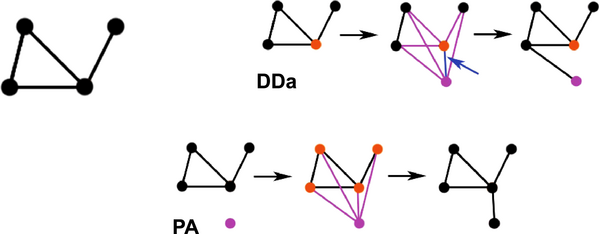
\epsfig{file=\fignet/RJH07-PLoSCompBiol-Fig7.ps, width=.4\textwidth,
        height=.3\textheight, bbllx=255, bblly=150, bburx=580,
        bbury=240, clip=} 
    \end{tabular}
  \end{tabular}
  
  \bigskip\Pause
  \paragraph{Likelihood.} Since the history of the network is not
  observed, the likelihood is a \emphase{sum over all possible paths}
  that could give raise to the observed network. \\
  \ra Direct ML can not be achieved.
  }

%====================================================================
\frame{ \frametitle{Inference}
  \paragraph{ABC inference:} See \Refer{O. Fran�ois}'s lecture
  yesterday. 

  \bigskip\Pause
  \paragraph{Network evolution.} ABC is based a pre-defined distance
  between the observed network $\Xbf$ and the simulated one $\Xbf'$
  $$
  d[S(\Xbf), S(\Xbf')].
  $$
  where $S(\Xbf)$ is the vector of \emphase{summary statistics}, e.g.
  \begin{itemize}
    \item number of edges,
    \item motifs counts ($\mathsf{V}$, $\nabla$, , etc.),
    \item ...
  \end{itemize}

  \bigskip\Pause
  \paragraph{Remarks.}
  \begin{enumerate}
    \item The proposed algorithm looks like a Metropolis-Hastings for a
    \emphase{ERGM with same statistics $S$ and fixed parameter
      $\gammabf$} (summarised in the choice of the distance).
    \item The calculation of the statistics $S$ for each simulated graph
    remains an \emphase{algorithmic issue}.
  \end{enumerate}
  }

%====================================================================
\section{Network topology}
\frame{ \frametitle{Network topology} }
%====================================================================
\subsection{Networks as random graphs}
%==================================================================== 
\frame{ \frametitle{Networks as random graphs}
  \paragraph{Aim:} 
  \begin{itemize}
  \item The global topology of the network give some insights about it
    \emphase{general behaviour and properties} (\refer{BaA99,AlB02}).
  \item \emphase{Mechanistic models} explaining the observed topology
    are not always available, or mathematically tractable.
  \item \emphase{'Null' or reference models} provide a naive and yet
  reasonably faithful description of the observed network.   
  \end{itemize}

  \bigskip\Pause
  \paragraph{Reference models}
  \begin{itemize}
  \item Provide a global picture of the network structure,
  \item Predict expected topologies for 'similar' networks,
  \item Provide a proper framework to simulate 'realistic' networks,
  \item Allow us to detect 'unexpected' structures in observed
    networks.
  \end{itemize} 

  \Pause
  \ra Similar to Markovian models in DNA sequence analysis (cf
  \Refer{S. Schbath} yesterday).

  }

%====================================================================
\subsection{Fitting network characteristics}
%==================================================================== 
\frame{ \frametitle{Some (simple) models fitting network characteristics}
  \paragraph{Density (number of edges):} The Erd�s \& R�nyi (ER)
  model states that 
  $$
  \{X_{ij}\}_{1 \leq i < j \leq n} \text{ i.i.d.}, \quad X_{ij}
  \sim \Bcal(\gamma) \qquad (\thetabf = \gamma)
  $$
  \emphase{$\rightarrow$} Does not fit other characteristics (degree
  distribution, diameter, etc.) of most real network.

  \bigskip\bigskip\Pause
  \paragraph{Colour frequencies (coloured networks):} Denoting $C_i$
  the colour of node $i$, the coloured Erd�s \& R�nyi (CER) model
  states that 
  $$
  \begin{array}{ll}
    \{C_i\}_{1 \leq i \leq n} \text{ i.i.d.}, & \quad C_i
    \sim \Mcal(1; \sbf=(s_1, s_2, \dots)) \\
    \{X_{ij}\}_{1 \leq i < j \leq n} \text{ i.i.d.}, & \quad X_{ij}
    \sim \Bcal(\gamma)
  \end{array}  
  \qquad (\thetabf = (\sbf, \gamma))
  $$
  }

%==================================================================== 
\frame{ \frametitle{Some (simple) models (cont'd)}
  \paragraph{Node degree:} Given $d_i =$ observed degree of
  node $i$, the fix degree distribution (FDD) models states that
  $$
  \Xbf \sim \Ucal\{\xbf: \sum_j x_{ij} = d_i\}
  \qquad (\thetabf = \dbf = \{d_i\})
  $$
  \emphase{$\rightarrow$} Sampling such graphs is not that easy (edge
  swapping algorithm). 

  \bigskip\bigskip\Pause
  \paragraph{Degree distribution.} Given $\dbf_{\obs} =
  \{d_i\}_i$ the degrees in the observed graph, the expected degree
  distribution (EDD) model states that
  $$
  \begin{array}{rcl}
    \{K_i\}_i \text{ i.i.d. } & \sim & \Ucal\{\dbf_{\obs}\} \\
    \{X_{ij}\} \text{ independent } | \{K_i\}: X_{ij}  & \sim &
    \Bcal(c K_i K_j)
  \end{array}
  \qquad (\thetabf = \dbf_{\obs})
  $$\Pause
  \paragraph{Similar to} permutation vs Markovian models for
  sequences. 

  \bigskip\bigskip\Pause
  \paragraph{Statistical inference:} Easy until now!
  }

%==================================================================== 
\frame{ \frametitle{Some (more complex) models}
  \bigskip
  \paragraph{Heterogeneity of connexion profiles:} Latent space models
  (\refer{BJR07}) suppose that each node $i$ occupies an
  \emphase{unknown latent position $Z_i$} and that
  $$
  \begin{array}{rcl}
    \{Z_i\} \text{ i.i.d. } & \sim & \pi \\
    \{X_{ij}\} \text{ independent } | \{Z_i\}: X_{ij}  & \sim &
    \Bcal[\gamma(Z_i, Z_j)]
  \end{array}
  \qquad (\thetabf = (\pi, \gamma))
  $$

  \Pause
  \paragraph{Continuous (\refer{HRH02}):} ($\simeq$ PCA)
  $$
  Z_i \in \Rbb^d, \qquad \text{logit}[\gamma(z, z')] = a - |z-z'|
  $$

  \Pause
  \paragraph{Discrete (\refer{NoS01}):} ($\simeq$ clustering, $=$
  mixture model)
  $$
  Z_i \in \{1, \dots, K\}, \qquad \gamma(k, \ell) = \gamma_{k\ell}.
  $$

  \Pause
  \paragraph{Statistical inference:} Not that easy
  \begin{itemize}
  \item Burdensome MCMC inference (limited to small networks)
  \item Variational approximation (\refer{DPR08}, see later)
  \item Variational Bayes inference
  \end{itemize}
  }

%==================================================================== 
\frame{ \frametitle{Some (more complex) models (cont'd)}
  \paragraph{Motif counts:} Exponential random graphs (ERGM, or $p^*$)
  (\refer{PaR07}) constitute a wide class of models stating that
  $$
  P(\Xbf; \thetabf) = \exp[\ubf(\Xbf)' \thetabf - c(\thetabf)]
  $$
  where $\ubf(\Xbf)$ is a vector of \emphase{sufficient statistics},
  e.g.
  $$
  \ubf(\Xbf) = \left[ \text{\# edges, \# $\Vsf$'s, \# triangles, \#
      3-stars, \dots} \right]
  $$\Pause
  \ra Statistical inference is \emphase{quite hard}. Ex:
  $$
  c(\thetabf) = \log \left(\sum_{\xbf} \exp[\ubf(\xbf)' \thetabf]\right).
  $$\Pause
  \emphase{$\rightarrow$} Motifs used in $\ubf(\Xbf)$ will
  \emphase{never be exceptional} w.r.t. this model.  
  }

%==================================================================== 
\subsection{Mixture Model}
%==================================================================== 
\frame{ \frametitle{Mixture Model} 
  \paragraph{Discrete-valued latent labels:}
  each node $i$ belong to class $q$ with probability $\pi_q$:
  $$
  \{Z_i\}_i \mbox{ i.i.d.}, \qquad Z_i \sim \Mcal(1; \pibf)
  $$
  where $\pibf = (\pi_1, \dots \pi_K)$;

  \bigskip\Pause
  \paragraph{Observed edges:} $\{X_{ij}\}_{i,
    j}$ are conditionally independent given the $Z_i$'s:
  $$
  (X_{ij} \;|\; Z_i = k, Z_j = \ell) \sim f_{k\ell}(\cdot).
  $$
  where $f_{k\ell}(\cdot)$ is some parametric distribution
  $f_{k\ell}(x) = f(x; \gamma_{k\ell})$, e.g.
  $$
  (X_{ij}|Z_{ik}Z_{j\ell}=1) \sim \Bcal(\gamma_{k\ell})
  $$
  We denote   $\gammabf = \{\gamma_{k\ell}\}_{k, \ell}.$
  
  \bigskip\Pause
  \paragraph{Inference:} We need to estimate
  $$
  \thetabf = (\pibf, \gammabf)
  \qquad \text{and} \qquad
  P(Z_i | \Xbf)
  $$
  }

%==================================================================== 
\frame{ \frametitle{Illustration: A social network}
  \vspace{-1cm}\hspace{-1cm}
  \begin{tabular}{c}
    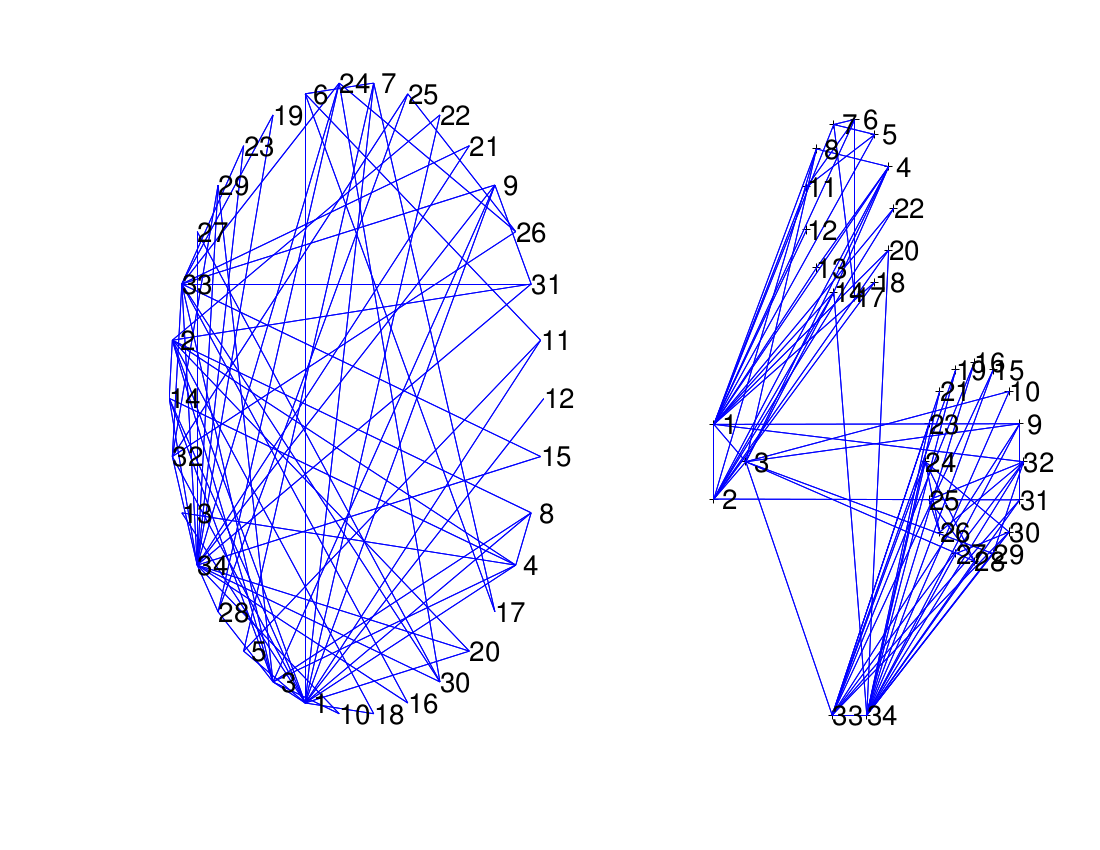
\epsfig{file = \fignet/Karate-Graph.eps, clip=, width=3.5cm,
      height=10cm, angle=270}
    \\
    \\
    \begin{tabular}{cc}
      \begin{tabular}{p{.45\textwidth}}
        \paragraph{Data.} Social binary network of friendship within a
        sport club. \\
        \\
        \paragraph{Results.} 
        The split is recovered and the role of the leaders is underlined. 
      \end{tabular}
      &
      \begin{tabular}{p{.5\textwidth}}
        {\small
          \begin{tabular}{c|rrrr}
            & \multicolumn{4}{c}{$\widehat{\gamma}_{k\ell}$ (\%)} \\
            $k / \ell$ &  {1} & 2 & 3 &  4 \\
            \hline
            {1} &  {100} &   {53} &  {16} & {16} \\  
            {2} & - &  {12} & {0} & {7}  \\  
            3 & - & - & 8 & 73 \\
            4 & - & - & - & 100\\
            \hline
            $n\pi_{\ell}$        & 3 &  13       & 16    & 2     \\
          \end{tabular}
          }
      \end{tabular}
    \end{tabular}
  \end{tabular}
  }

%==================================================================== 
\subsection{Variational Inference}
%==================================================================== 
\frame{ \frametitle{Maximum likelihood inference}
  \paragraph{Maximum likelihood estimate:} We are looking for
  $$
  \widehat{\thetabf} = \arg\max_{\thetabf} \log P(\Xbf; \thetabf)
  $$\Pause

  \paragraph{Incomplete data model:}
  \begin{itemize}
  \item $
    P(\Xbf; \thetabf) = \sum_{\Zbf} P(\Xbf, \Zbf; \thetabf)
    $
    is generally not always computable.
  \item This of 
    $
    P(\Xbf, \Zbf; \thetabf)
    $
    is much easier ... except that {$\Zbf$ is unknown}.
  \end{itemize}
%   }

% %==================================================================== 
% \frame{ \frametitle{Variational approach}
  \bigskip\Pause
  \paragraph{Lower bound of the log-likelihood:}
  For any distribution $Q(\Zbf)$, we have (\refer{JGJ99,Jaa00})
  \begin{eqnarray*}
    \log P(\Xbf) & \geq & \log P(\Xbf) - KL[Q(\Zbf); P(\Zbf|\Xbf)] \\
%     & = & \log P(\Xbf) - \int Q(\Zbf) \log Q(\Zbf) \dd\Zbf + \int
%     Q(\Zbf) \log \emphase{P(\Zbf |\Xbf)} \dd\Zbf \\   
%     & = & - \int Q(\Zbf) \log Q(\Zbf) \dd\Zbf + \int Q(\Zbf) \log
%     \emphase{P(\Xbf, \Zbf)} \dd\Zbf \\
    & = & \Hcal(Q) + \Esp_Q[\log P(\Xbf, \Zbf)] \\
    \text{where} \qquad\qquad
    \Hcal(Q) & = & \int Q(\Zbf) \log Q(\Zbf) \dd\Zbf \\
    \Esp_Q[\log P(\Xbf, \Zbf)] & = & \int Q(\Zbf) \log
    \emphase{P(\Xbf, \Zbf)} \dd\Zbf 
  \end{eqnarray*}
  }

%==================================================================== 
\frame{ \frametitle{2 cases}
  \paragraph{If $P(\Zbf|\Xbf)$ can be calculated}: taking $Q(\Zbf) =
  P(\Zbf|\Xbf)$ achieves the maximisation of $\log P(\Xbf)$ through
  this of
  $$
  \Esp_Q[\log P(\Xbf, \Zbf; \thetabf)].
  $$
  \emphase{$\rightarrow$} E-M algorithm for independent mixtures, hidden
  Markov models, etc. %(\refer{DLR77,MaP00,CMR05}).
  
  \bigskip\bigskip\Pause
  \paragraph{If $P(\Zbf|\Xbf)$ can not be calculated}: the best lower
  bound of $\log P(\Xbf)$ is obtained for
  $$
  Q^* = \arg\min_{Q \in \Qcal} KL[Q(\Zbf); P(\Zbf|\Xbf)]
  $$
  \emphase{$\rightarrow$} Mean-field approximation for random graphs.
  }

%====================================================================
\frame{ \frametitle{Variational E-M}
  \paragraph{'Expectation' step (E-step):} calculate
  $$
  P(\Zbf|\Xbf; \thetabf)
  $$
  or its approximation
  $$
  Q^* = \arg\min_{Q \in \Qcal} KL[Q(\Zbf); P(\Zbf|\Xbf; \thetabf)].
  $$

  \bigskip
  \paragraph{Maximisation step (M-step):} estimate $\thetabf$ with
  $$
  \widehat{\thetabf} = \arg\max_{\thetabf} \Esp_Q[\log P(\Xbf, \Zbf; \thetabf)]
  $$
  which maximise $\log P(\Xbf)$ if $Q(\Zbf) = P(\Zbf|\Xbf)$, and its
  lower bound otherwise.
  }

%==================================================================== 
\frame{ \frametitle{Back to networks}
  \paragraph{Dependency structure.}

  \bigskip
  \begin{tabular}{c|c|c}
    \begin{tabular}{p{.28\textwidth}}
      \emphase{Graphical rep.:} \\ 
      $P(\Zbf) P(\Xbf|\Zbf)$
    \end{tabular}
    &
    \begin{tabular}{p{.28\textwidth}}
      \emphase{Moral graph}  \\
      (\refer{Lau96})
    \end{tabular}
    &
    \begin{tabular}{p{.28\textwidth}}
      \emphase{Cond. dependency:} \\ 
      $P(\Zbf|\Xbf)$
    \end{tabular}
    \\
    \hline
    & & \\
    \begin{tabular}{c}
      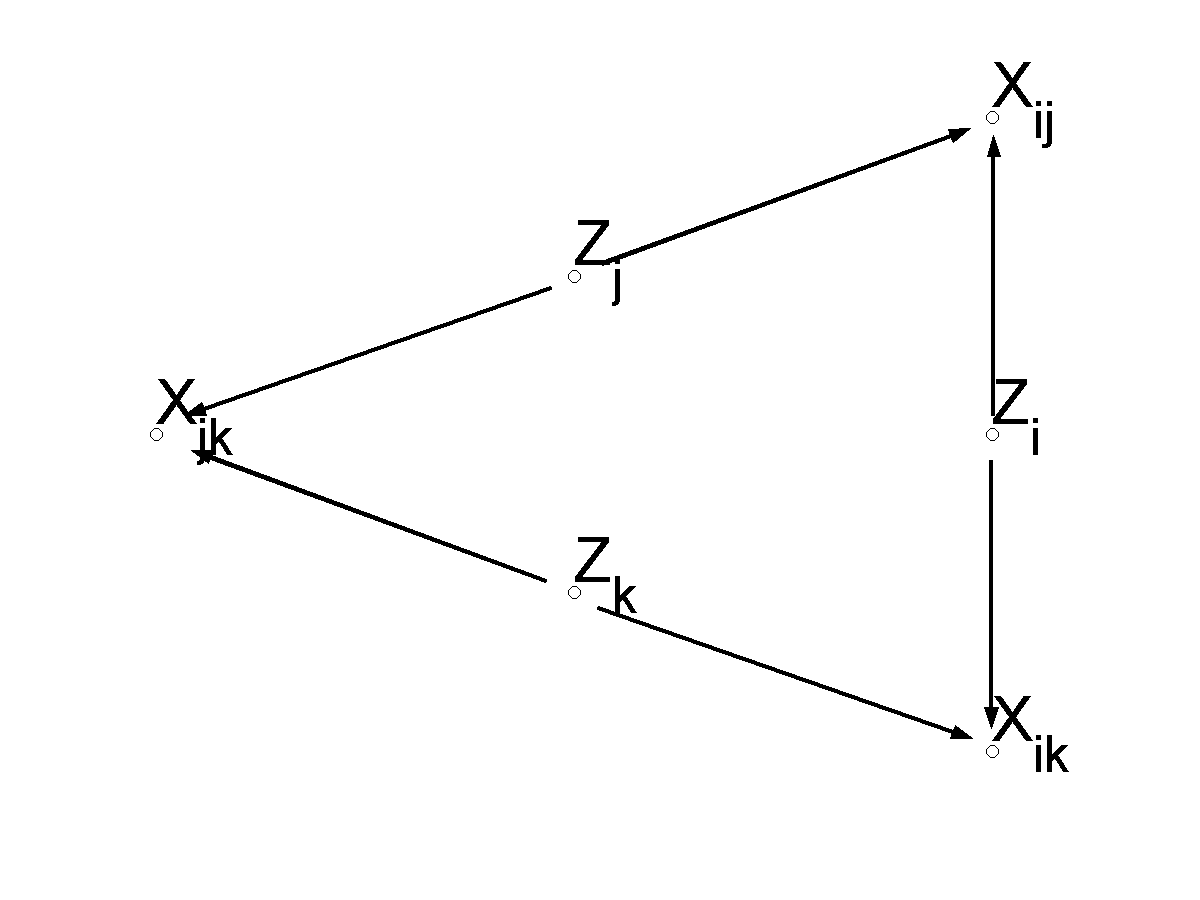
\epsfig{file=\fignet/FigNetworks-DepGraph,
      width=.25\textwidth, clip=} 
    \end{tabular}
    & 
    \begin{tabular}{c}
      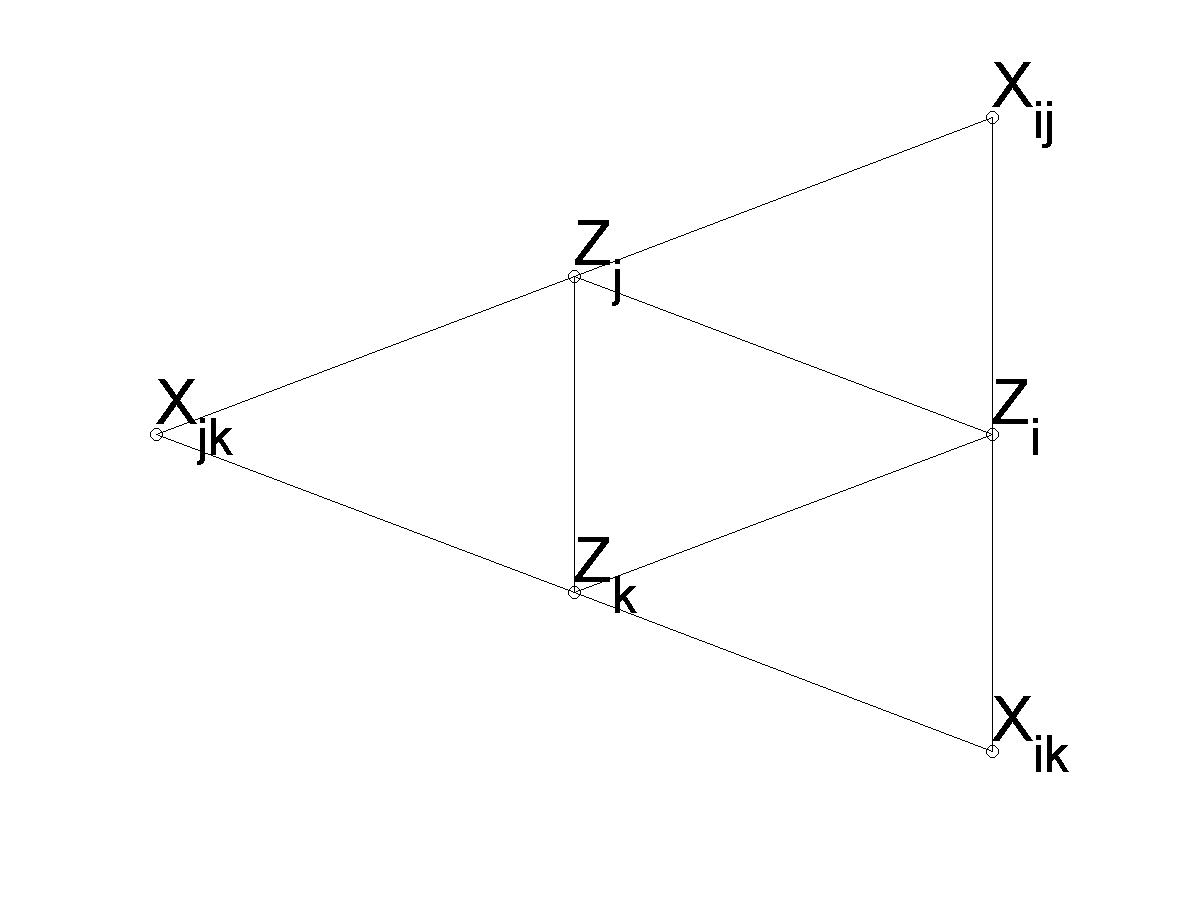
\epsfig{file=\fignet/FigNetworks-DepGraph-Moral,
      width=.25\textwidth, clip=}
    \end{tabular}
    & 
    \begin{tabular}{c}
      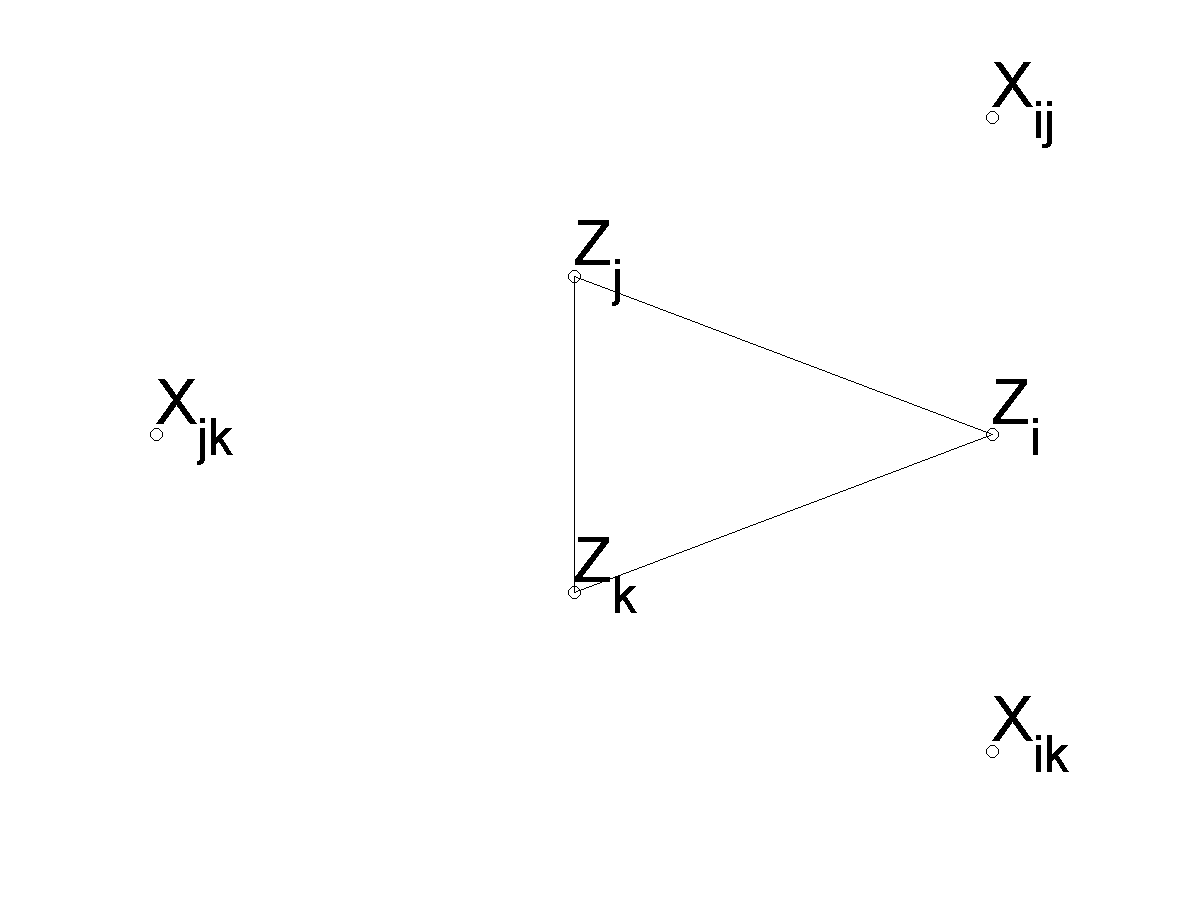
\epsfig{file=\fignet/FigNetworks-DepGraph-Conditional,
      width=.25\textwidth, clip=}
    \end{tabular} 
  \end{tabular}
  
  \bigskip\bigskip\Pause
  The conditional dependency of $\Zbf$ is a \emphase{clique} \\
  \ra no factorisation can be hoped to calculate $P(\Zbf|\Xbf)$
  (unlike hidden Markov random fields)\\ 
  \ra $P(\Zbf|\Xbf)$ can {only be approximated}.  
  }
%====================================================================
\frame{ \frametitle{Likelihood}
  \paragraph{Complete log-likelihood:}
  $$
  \log P(\Xbf, \Zbf) = \sum_{i, k} Z_{ik} \log \pi_k + \sum_{i, j}
  \sum_{k, \ell} Z_{ik} Z_{j\ell} \log f(X_{ij}; \gamma_{k\ell}).
  $$
   
  %\bigskip
   \paragraph{'Completed' log-likelihood:} 
   $$
   \Esp_Q[\log P(\Xbf, \Zbf)] = \sum_{i, k}
   \underset{\emphase{\normalsize
       \tau_{ik}}}{\underbrace{\Esp_Q[Z_{ik}]}} \log \pi_k + \sum_{i,
     j} \sum_{k, \ell} \Esp_Q[Z_{ik} Z_{j\ell}]  \log f(X_{ij};
   \gamma_{k\ell}). 
   $$
   
   ~\\
   \paragraph{M-step:} weighted version of the MLE.  
   }

%====================================================================
\frame{ \frametitle{Approximation of $P(\Zbf|\Xbf)$}
  \paragraph{Problem:}  
  We are looking for
  $$
  Q^* = \arg\min_{Q \in \Qcal} KL[Q(\Zbf); P(\Zbf|\Xbf)].
  $$

  \Pause
  \begin{itemize}
%   \item The optimum over all possible distributions is
%     \emphase{$Q^*(\Zbf) = P(\Zbf|\Xbf)$} ... which can no be
%     calculated.
  \item We restrict ourselves to the set of \emphase{factorisable
      distributions}:
    $$
    \Qcal = \left\{Q: Q(\Zbf) = \prod_i Q_i(Z_i) = \prod_i \prod_k
      \tau_{ik}^{Z_{ik}}\right\}. 
    $$
    $Q^*$ is characterised by the set of optimal parameters
    $\tau_{ik}^*$'s:
    $$
    \emphase{\tau_{ik}^* = \Esp_Q[Z_{ik}] \approx \Pr\{Z_i=k|\Xbf\}}.
    $$  \Pause
  \item The optimal $\tau_{ik}^*$'s can be found using {standard
    (constrained) optimisation} techniques.
  \end{itemize}
  }
    
%====================================================================
\frame{ \frametitle{Best factorisable approximation}
  The optimal $\tau_{ik}$'s must satisfy
%   $$
%   \left.\frac{\partial}{\partial
%       \tau_{ik}}\right|_{\{\tau_{ik}^*\}} \left\{KL[Q(\Zbf);
%     P(\Zbf|\Xbf)] + \sum_i \lambda_i \left(\sum_{k} \tau_{ik} -
%       1\right)\right\} = 0
%   $$
%   which leads to 
  the {fix-point relation}:
  $$
  \tau_{ik}^* \propto \pi_k \prod_{j \neq i} \prod_\ell
%   \left[\gamma_{k\ell}^{X_{ij}} (1 -
%     \gamma_{k\ell})^{1-X_{ij}}\right]^{\emphase{\tau^*_{j\ell}}}
  f_{k\ell}(X_{ij})^{\emphase{\tau^*_{j\ell}}}
  $$
  also known as \emphase{mean-field} approximation in physics.

  \bigskip
  \paragraph{Intuitive interpretation:}
  $$
  \Pr\{Z_i=k | \Xbf, \Zbf_{\emphase{\setminus i}}\} \propto \pi_k
%   \prod_{j \neq i} \prod_\ell \left[\gamma_{k\ell}^{X_{ij}} (1 -
%     \gamma_{k\ell})^{1-X_{ij}}\right]^{\emphase{Z_{j\ell}}}.
  \prod_{j \neq i} \prod_\ell
  f_{k\ell}(X_{ij})^{\emphase{Z_{j\ell}}}. 
  $$

  \bigskip
  \paragraph{Improvement:} The approximation of $\Esp_Q[Z_{ik}
  Z_{j\ell}]$ can be improved via a \emphase{message passing
    algorithm}.  
  }

%====================================================================
\subsection{Application to regulatory networks}
\frame{ \frametitle{Application to regulatory network}
%==================================================================== 
  \vspace{-.5cm}\hspace{-.5cm}
  \begin{tabular}{ll}
    \begin{tabular}{p{6cm}}
      Regulatory network = directed graph where
      \begin{itemize}
      \item \emphase{Nodes =} genes (or groups of genes, e.g. operons)
      \item \emphase{Edges =} regulations:
        $$
        \emphase{\{i \rightarrow j\}}
        \quad \Leftrightarrow \quad 
        \emphase{i \text{ regulates } j}
        $$
      \end{itemize}

      Typical questions are
      \begin{itemize}
      \item Do some nodes share similar connexion profiles?
      \item Is there a 'macroscopic' organisation of the network?
      \end{itemize}    
    \end{tabular}
    &
    \begin{tabular}{l}
      \hspace{-.75cm}
      \epsfig{file=\fignet/im_EcoliVEM_2.ps,
      width=.45\textwidth, clip=} 
    \end{tabular}
  \end{tabular}
  }

%==================================================================== 
\frame{ \frametitle{Meta-graph representation}
  \hspace{-0.75cm}
  \begin{tabular}{cc}
    \begin{tabular}{p{0.45\textwidth}}
      \epsfig{file=\fignet/im_EcoliVEM.ps,
      width=.45\textwidth, clip=} 
    \end{tabular}
    &
    \begin{tabular}{p{0.45\textwidth}}
      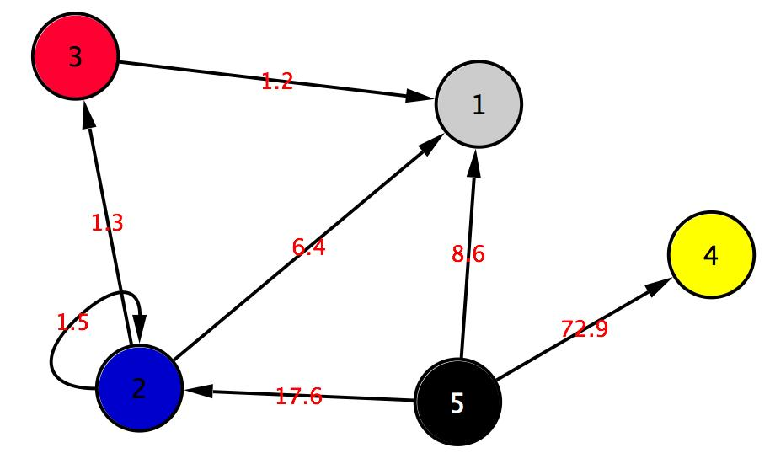
\epsfig{file=\fignet/VEMmetagraphe.ps,
      width=.45\textwidth, clip=}  
      \\ \\
      \tiny{$\begin{array}{cccccc}
          \widehat{\gamma}_{k\ell}~(\%) & 1 & 2 & 3 & 4 & 5 \\
          \hline
          1 & . & . & . & . & . \\
          2 & 6.40 & 1.50 & 1.34 & . & . \\
          3 & 1.21 & . & . & . & . \\
          4 & . & . & . & . & . \\
          5 & 8.64 & 17.65 & . & 72.87 & 11.01 \\
          \hline
          \widehat{\alpha}~(\%) & 65.49 & 5.18 & 7.92 & 21.10 & 0.30
        \end{array}$}
      \\ \\
      (source \refer{PMD09})
    \end{tabular}
  \end{tabular}
  }

%==================================================================== 
\subsection{Variational approximation for networks}
%==================================================================== 
\frame{ \frametitle{Variational Bayes inference}
  \paragraph{Bayesian setting:} Both $\thetabf$ and $\Zbf$ are
  unobserved and we want to retrieve $P(\Zbf, \thetabf|\Xbf)$

  \bigskip
  \paragraph{Exponential family / conjugate prior:} if
  \begin{eqnarray*}
    P(\thetabf) & \propto & \exp[\phi(\thetabf)' \nubf] \\
    P(\Xbf, \Zbf | \thetabf) & \propto & \exp[\phi(\thetabf)' u(\Xbf, \Zbf)]
  \end{eqnarray*}
  the best approximate distribution  
  $$
  Q^* = \arg\min_{Q \in \Qcal} KL[Q(\Zbf, \thetabf); P(\Zbf,
  \thetabf[\Xbf)]
  $$
  within the class of factorisable distributions $\Qcal$:
  $$
  \Qcal = \{Q: Q(\Zbf, \thetabf) = Q_Z(\Zbf)Q_\theta(\thetabf)\}
  $$
  can be recovered via a \emphase{variational Bayes E-M algorithm (VBEM)}
  (\refer{BeG03}). 
  }

%==================================================================== 
\frame{ \frametitle{VB-EM} 
  
  The optimal $Q^*(\Zbf, \thetabf) = Q^*_Z(\Zbf)Q^*_\theta(\thetabf)$
  can be recovered by an EM-like algorithm
  \begin{eqnarray*}
    \text{\emphase{M step:}} \qquad \log Q_{\thetabf}(\thetabf) & = &
    \phi(\thetabf)^\intercal \left\{\Esp_{Q_Z}[u(\Xbf, \Zbf)] +
      \nubf\right\} + \cst \\ 
    \\
    \text{\emphase{'E' step:}} \qquad \log Q_Z(\Zbf) & = &
    \Esp_{Q_\theta}[\phi(\thetabf)]^\intercal u(\Xbf, \Zbf) + \cst
  \end{eqnarray*}

  \bigskip
  \paragraph{Mean-field approximation.} For network mixture models, we get
  \begin{eqnarray*}
    \tau_{iq}^{\VBEM} &\propto&
    e^{\psi(\widetilde{n_q})-\psi\left(\sum_{l=1}^Q
        \widetilde{n}_\ell\right)} \prod_{j \neq i}^n \prod_{l=1}^Q
    e^{\tau_{j\ell}^{\VBEM} \left\{\psi(\widetilde{\zeta}_{q\ell}) -
        \psi(\widetilde{\eta}_{q\ell} + \widetilde{\zeta}_{q\ell}) +
        X_{ij}
        [\psi(\widetilde{\eta}_{q\ell})-\psi(\widetilde{\zeta}_{q\ell})]
      \right\})}    
  \end{eqnarray*}
  }

%==================================================================== 
\frame{ \frametitle{VB-EM Credibility intervals}
  \paragraph{VB-EM Credibility intervals} with a mixture of 2 groups of nodes\\
  ~\\
  \includegraphics[width=1\textwidth]{\fignet/im-ICQ2-2-new} \\
  $\pi_1$: $+$, $\gamma_{11}$: \textcolor{red}{$\triangle$},
  $\gamma_{12}$: \textcolor{blue}{$\circ$}, $\gamma_{22}$:
  \textcolor{green}{$\bullet$}

  \begin{itemize}
  \item For all parameters, VB-EM posterior credibility intervals
    achieve the nominal level (90\%), as soon as $n \geq 25$.
  \item $\rightarrow$ the VB-EM approximation works well, at least for
    graphs.
  \end{itemize}
  }

%==================================================================== 
\frame{ \frametitle{Convergence rate of the {\VBEM} estimates}
  \emphase{Width of the posterior credibility intervals.}
  {$\alpha_1$}, \textcolor{red}{$\pi_{11}$},
  \textcolor{blue}{$\pi_{12}$}, \textcolor{green}{$\pi_{22}$}
  \\
  \includegraphics[width=1\textwidth]{\fignet/im-ICQ2-3} \\

  \begin{itemize}
  \item The width decreases as $1/\sqrt{n}$ for $\alpha_1$.
  \item It decreases as $1/n$ for $\pi_{11}$, $\pi_{12}$ and
    $\pi_{22}$.
  \item Consistent with the penalty of the ICL criterion
    of \refer{DPR08}: 
    $$
    (Q-1)\log n + Q^2 \log[n(n-1)/2].
    $$
  \end{itemize}
  }

%==================================================================== 
\frame{ \frametitle{Variational approximation for graphs}

  The quality of the inference based on the variational approximation is
  not very well known yet.
  \begin{itemize}
  \item VEM algorithm converge to a \emphase{different optimum than
      ML} in the general case (\refer{GuB05}), except for degenerated
    models.
  \item Consistency is proved for \emphase{some incomplete data models}
    (\refer{McT09}).
  \item VB-EM often under-estimate the posterior variances.
  \end{itemize}

  \bigskip\Pause
  \paragraph{Specific case of graphs.}
  \begin{itemize}
  \item Specific asymptotic framework \emphase{$'p' = n$}.
  \item Mean field approximation asymptotically exact for some models
    with infinite range dependency (\refer{OpW01}: law of large number
    argument).
  \item Network mixtures are, in some sense, degenerated: 
    $
    \Pr\{\widehat{\Zbf} = \Zbf\} \longrightarrow 1.
    $
    \Refer{Celisse \& Daudin}
  \end{itemize}
  }

%====================================================================
\section{Network motifs}
\frame{\frametitle{Network motifs}}
%====================================================================
\subsection{What motifs?}
\frame{ \frametitle{What motifs?}

  \begin{tabular}{ll}
    \begin{tabular}{p{0.8\textwidth}}
      \paragraph{Local patterns} constitute 
      {functional modules} or basic building
      blocks of complex networks (\refer{SMM02}). \\

      ~\\
      \paragraph{Transcription regulatory networks:} 
      motifs may perform specific regulatory functions
      (e.g. feed-forward loop, bi-fan: see right). \\
     \refer{MSI02}, \refer{MaA03}, \refer{PIL05}
 
      ~\\
      \paragraph{Metabolic motif} may reveal systematic associations of
      reactions in metabolic pathways. \\
      \refer{LFS06}
    \end{tabular}
    &
    \hspace{-0.5cm}
    \begin{tabular}{p{0.2\textwidth}}
      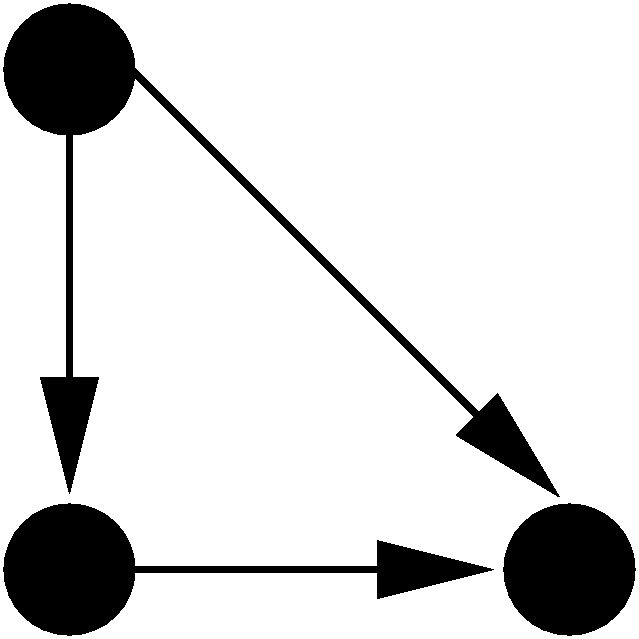
\epsfig{file=\fignet/feedforwardloop.eps, clip=,
        width=.1\textwidth} \\
      \\
      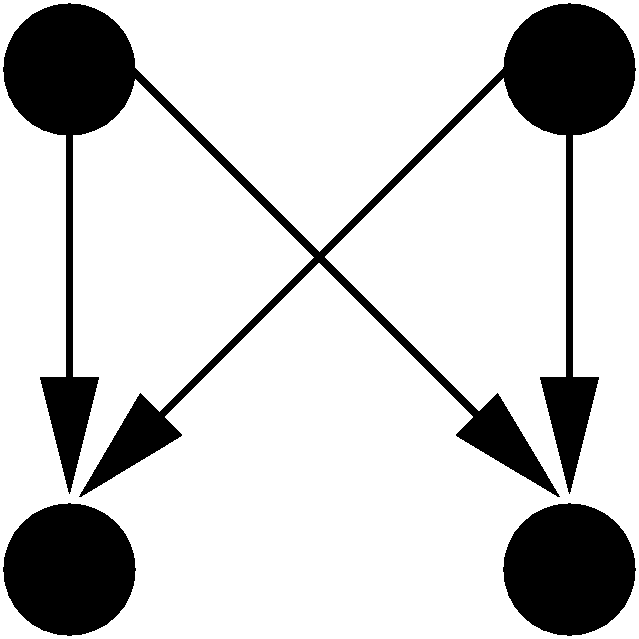
\epsfig{file=\fignet/bifan.eps, clip=, width=.1\textwidth}
    \end{tabular}
  \end{tabular}
  }

%==================================================================== 
\subsection{2 different motifs}
%====================================================================
\frame{\frametitle{Coloured motif in metabolic networks}
  \begin{tabular}{cc}
    \begin{tabular}{p{0.45\textwidth}}
      A motif $\mbf$ is defined by a set of $k$ colors (with possible
      repetitions). \\
      ~\\
      \emphase{Colour} = Enzyme classification\\
      ~\\    
      A coloured motif $\mbf$ of size $k$ occurs when
      \begin{itemize}
      \item a set of $k$ nodes
      \item composing a \emphase{connected} subgraph
      \item with \emphase{prescripted} colors
      \end{itemize}
      is observed. \\
    \end{tabular}
    &
    \begin{tabular}{p{0.45\textwidth}}
      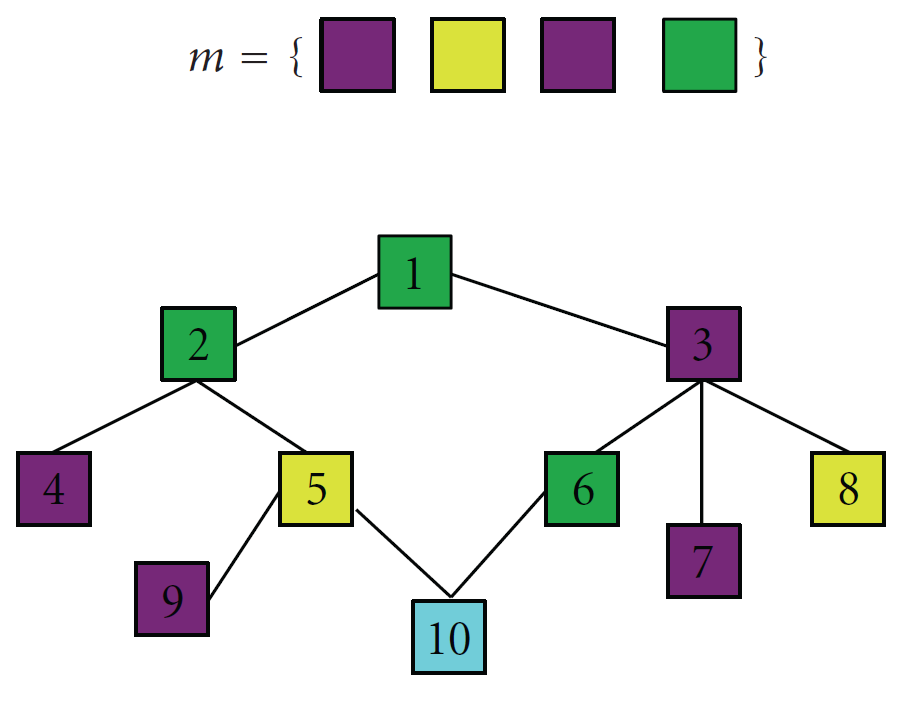
\includegraphics[width=.45\textwidth]{\fignet/SLS09-JBSB-Fig2}
      \\
      \\
      3 occurrences of the motif $m$. \\
      \\
      (\refer{SLS09})
    \end{tabular}
  \end{tabular}
  }

%==================================================================== 
\frame{\frametitle{Topological motif in gene-interaction networks}
  \paragraph{Definition.}  A topological motif $\mbf$ of is
  characterised by its adjacency matrix (also denoted by $\mbf$):
  $$
  m_{uv} = \Ibb\{u \sim v\}.
  $$

  \hspace{-0.7cm}
  \begin{tabular}{cc}
    \begin{tabular}{p{0.4\textwidth}}
      \paragraph{Permutations.} For a given motif $\mbf$, we need to
      consider the set $\Rcal(\mbf)$ of its permutations. \\
      \\
      \paragraph{Right:} the $\mathsf{V}$ motif may occure in 3 ways at a
      {fixed} position $\alpha = (i,j,k)$: \\
      \\
    \end{tabular}
    &
    \begin{tabular}{ccc}
      $\mbf$ &  $\mbf^{\prime}$ & $\mbf^{\prime \prime}$ \\
      & & \\
      $\tiny{\left[ \begin{array}{ccc} 
          0 & 1 & 1 \\ . & 0 & 0 \\ . & . & 0 
        \end{array} \right]}$  &
      $\tiny{\left[ \begin{array}{ccc} 
          0 & 1 & 0 \\ . & 0 & 1 \\ . & . & 0 
        \end{array} \right]}$ &
      $\tiny{\left[ \begin{array}{ccc} 
          0 & 0 & 1 \\ . & 0 & 1 \\ . & . & 0 
        \end{array} \right]} $ \\
      &&
      \\
      \epsfig{file=\fignet/version2.eps, width=0.1\textwidth} & 
      \epsfig{file=\fignet/version3.eps, width=0.1\textwidth} & 
      \epsfig{file=\fignet/version1.eps, width=0.1\textwidth} 
      \\
    \end{tabular}
  \end{tabular}
  }

%====================================================================
\frame{\frametitle{Occurence of a topological motif}
  \begin{tabular}{cc}
    \begin{tabular}{p{0.45\textwidth}}
      A topological motif $m$ of size $k$ occurs when
      \begin{itemize}
      \item a set of $k$ nodes
      \item with \emphase{prescripted} edges
      \end{itemize}
      is observed. \\
      ~\\
      So-called 
      $$
      \text{\emphase{induced motif}}
      $$
      $\neq$ exact occurrence.
    \end{tabular} 
    &
    \begin{tabular}{p{0.45\textwidth}}
      \includegraphics[width=.3\textwidth]{\fignet/PDK08-JCB-Fig1}
      \\
      \\
      1 occurrence of '$\nabla$'\\
      and 5 occurrences '$\Vsf$'. \\
      \\
      (\refer{PDK08})
    \end{tabular}
  \end{tabular}
  }

%====================================================================
\subsection{Motif count}
%====================================================================
\frame{\frametitle{Motif occurrence}
  \paragraph{Position.} A ($k$-)position $\alpha$ is a set of $k$
  different nodes taken is ascending order:
  $$
  \alpha = (i_1, ... i_k), \qquad i_1 < i_2 < ... < i_k.
  $$
  A graph of size $n$ contains \emphase{$\displaystyle{\binom{n}{k}}$
    positions}. 
  
  \bigskip\bigskip
  \paragraph{Motif occurrence:} Binary variable $Y_{\alpha}(\mbf) =
  \Ibb\{\mbf \text{ occurs at } \alpha\}$ \\ \Pause
  ~\\
  \begin{tabular}{p{0.55\textwidth}p{0.4\textwidth}}
    \hspace{-0.3cm}
    \paragraph{Coloured motif:} 
    \begin{eqnarray*}
      Y_{\alpha}(\mbf) & = & \Ibb\{\text{$C_\alpha = \mbf$}\} \\ 
      & \times & \Ibb\{\text{sub-graph $\Xbf_\alpha$
        connected}\}
    \end{eqnarray*} \Pause
    &
    \hspace{-0.3cm}
    \paragraph{Topological motif:} 
    $$
    Y_{\alpha}(\mbf) = \prod_{1 \leq u < v \leq k}
    (X_{i_ui_v})^{m_{uv}} 
    $$ 
    (induced occurrence)  
  \end{tabular}
  }

%====================================================================
\frame{\frametitle{Occurrence probability}
  \paragraph{Two assumptions (\refer{PDK08}):} 
  \begin{enumerate}[(H1)]
  \item {Stationarity:} (not true for FDD)
    $$ 
    \Dcal(X_{i_1j_1}, \ldots, X_{i_{\ell}j_{\ell}}) = \Dcal
    (X_{i'_1j'_1}, \ldots, X_{i'_{\ell}j'_{\ell}}). 
    $$
  \item {Independence of disjoint occurrences:}
    $$
    Y_\alpha(\mbf) \perp Y_\beta(\mbf) \quad \text{ if } \quad \alpha
    \cap \beta =\emptyset.  
    $$
  \end{enumerate}

  \bigskip\bigskip\Pause
  \paragraph{Occurrence probability:} 
  Under (H1), $\Pr\{Y_\alpha=1\}$ does not depend on $\alpha$:
  $$
  \forall \alpha, \forall \mbf' \in \Rcal(\mbf), \qquad
  \Pr\{Y_{\alpha}(\mbf') = 1\} = \Pr\{Y_{\alpha}(\mbf) = 1\} = \mum.
  $$
  }

%==================================================================== 
\frame{ \frametitle{Occurrence probability (cont'd)}
  \begin{tabular}{p{0.5\textwidth}p{0.5\textwidth}}
    \paragraph{Coloured motif:} 

    {Coloured Erd�s-Renyi (CER):}
    $$
    \mum =  {f(\mbf)} {g(k, p)}
    $$
    where 
    \begin{itemize}
    \item 
      $f(\mbf) = \Pr\{\text{\emphase{colors}}\}$
      $$
      = \frac{k!}{\prod_c s(c)!} \prod_i f(m_i)
      $$
    \item $g(k, \gamma) = \Pr\{\text{\emphase{connectedness}}\}$: $1 - g(k,
      \gamma) =$
      $$
      \sum_{i=1}^{k-1} \binom{k-1}{i-1} g(i, \gamma) (1-\gamma)^{i(k-i)}
      $$ 
    \end{itemize}
    \Pause
    &
    \paragraph{Topological motif:} 

    {Erd�s-Renyi (ER):}
    $$
    \mum = \prod_{1 \leq u<v \leq k} \gamma^{m_{uv}}.
    $$\Pause
    {Expected degree distribution (EDD):} 
    $$
    \mum \propto \prod_{u=1}^k \Esp\left(D^{m_{u+}} \right).
    $$\Pause
    {Mixture model:}
    \begin{eqnarray*}
      \mum   & =   & \sum_{c_1=1}^{Q} \hdots \sum_{c_k=1}^{Q}
      \alpha_{c_1}\hdots \alpha_{c_k} \\ 
      & & \times \prod_{1 \leq u<v \leq k} \gamma_{c_u,c_v}^{m_{uv}}.
    \end{eqnarray*}
  \end{tabular}
  
  }

%====================================================================
\subsection{(Exact) Moments of the count}
%====================================================================
\frame{\frametitle{Count}
  \paragraph{Count.} The total number of occurrences is the sum over
  {all positions} (and {all permutations}) of the binary variables: \\
  ~\\
  \begin{tabular}{p{0.4\textwidth}p{0.5\textwidth}}
    \paragraph{Coloured motif:} 
    $$
    N(\mbf) = \sum_{\alpha} Y_{\alpha}(\mbf)
    $$
    &
    \paragraph{Topological motif:} 
    $$
    N(\mbf) = \sum_{\alpha} \sum_{\mbf' \in \Rcal(\mbf)} Y_{\alpha}(\mbf')
    $$
  \end{tabular}

  \bigskip\Pause
  \paragraph{Counting the occurrences} in a given network is a
  non-trivial algorithmic task for both motifs:
  \begin{itemize}
  \item coloured (\refer{LFS06});
  \item topological (\refer{WeR06}, \refer{SMM02}).
  \end{itemize}

  \bigskip\Pause
  \paragraph{Other types of exceptionality} can be considered, such as
  local concentration of occurrences (\refer{Bir09b})

  
  }

%==================================================================== 
\frame{ \frametitle{Moments}
  \paragraph{Mean:} Straightforwardly
  $$
  \Esp_{col} N(\mbf) = \binom{n}{k} \mum,
  \qquad
  \Esp_{topo} N(\mbf) = \binom{n}{k} |\Rcal(\mbf)| \mum .
  $$

  \bigskip\Pause
  \paragraph{Variance:} Obtained via the calculation of $\Esp
  [N(\mbf)^2]$.
  \begin{eqnarray*}
    N^2(\mbf) & = & \sum_{\alpha, \beta \in I_k}
    \sum_{\mbf^\prime, \mbf''\in \mathcal{R}(\mbf)}
    Y_{\alpha}(\mbf')Y_{\beta}(\mbf'') \\
    \text{\emphase{if topological}}& = & \sum_{s=0}^k \sum_{|\alpha
    \cap \beta| = s} \sum_{\mbf', \mbf'' \in \Rcal(\mbf)} Y_{\alpha
    \cup \beta}(\mbf' \Omegas \mbf'')
  \end{eqnarray*}
  where $\Omegas$ is the \emphase{overlapping operator} with $s$
  common nodes and $\mbf' \Omegas \mbf''$ is the \emphase{super-motif}
  made of two overlapping occurrences of $\mbf'$ and $\mbf''$.
  }

%==================================================================== 
\frame{ \frametitle{Overlaps of coloured motifs}
  We have to calculate
  \begin{eqnarray*}
    \Esp [Y_\alpha(\mbf) Y_\beta(\mbf)] & \propto  &
    \Pr\{(\Xbf_\alpha \text{ connected}) \cap (\Xbf_\beta \text{
    connected}) \} \\
  & \emphase{\neq} & \Pr\{\Xbf_{\alpha \cup \beta} \text{ connected}\} = g(2k-s, \gamma)
  \end{eqnarray*}
    
%   The calculation of 
%   $\Esp Y_{\alpha \cup \beta}(\mbf\Omegas \mbf)$ is based on this of 
%   $$
%   \Pr\{(\Xbf_\alpha \text{ connected}) \cap (\Xbf_\beta \text{
%     connected}) \} 
%   $$
%   for overlapping positions $\alpha$ and $\beta$.

  \bigskip
  \noindent
  \begin{tabular}{cc}
    \hspace{-0.5cm}
    \begin{tabular}{p{0.4\textwidth}}
      This 
%       is different from
%       $$
%       \Pr\{\Xbf_{\alpha \cup \beta} \text{ connected}\} = g(2k-s, \gamma)
%       $$
%       and 
      requires to explore all possibilities for the \emphase{shared edges}.
      
      \bigskip
      \paragraph{Right:} Example for a motif $\mbf$ of size $k =2$ and
      $s=1$. \\
    \end{tabular}
    &
    \hspace{-0.5cm}
    \begin{tabular}{p{0.6\textwidth}}
      \includegraphics[width=.5\textwidth,
      height=0.4\textheight]{\fignet/SLS09-JBSB-Fig3} 
    \end{tabular}
  \end{tabular}
  }

%==================================================================== 
\frame{ \frametitle{Overlaps of topological motifs}
  \hspace{-0.5cm}
  \begin{tabular}{cc}
    \begin{tabular}{p{0.4\textwidth}}
      \paragraph{Super-motifs} are made of overlapping
      occurrences of equivalent versions of $\mbf$. \\
      \\ 
      The adjacency matrices of all super-motifs can be
      \emphase{systematically enumerated}. \\ 
%      \\
%       The algorithm consist in the systematic exploration of all $\mbf'
%       \Omegas \mbf''=$ 
%       $$
%       \left(\begin{array}{c|c|c}
%           \mbf'_{11} & \mbf'_{12} & \Obf \\
%           \hline
%           \mbf'_{21} & \max(\mbf'_{22}, \mbf''_{11}) &  \mbf''_{12} \\
%           \hline
%           \Obf  & \mbf''_{21} &  \mbf''_{22} \\
%         \end{array} \right).
%       $$
      \\
      \paragraph{Right:} All $\mbf' \Omegas \mbf''$ with $s=3$
      for the 4 spike star motif: \\
      \centerline{\begin{tabular}{cc}
          \begin{tabular}{c} $\mbf = $ \end{tabular} & 
          \begin{tabular}{c} \hspace{-1cm}     
            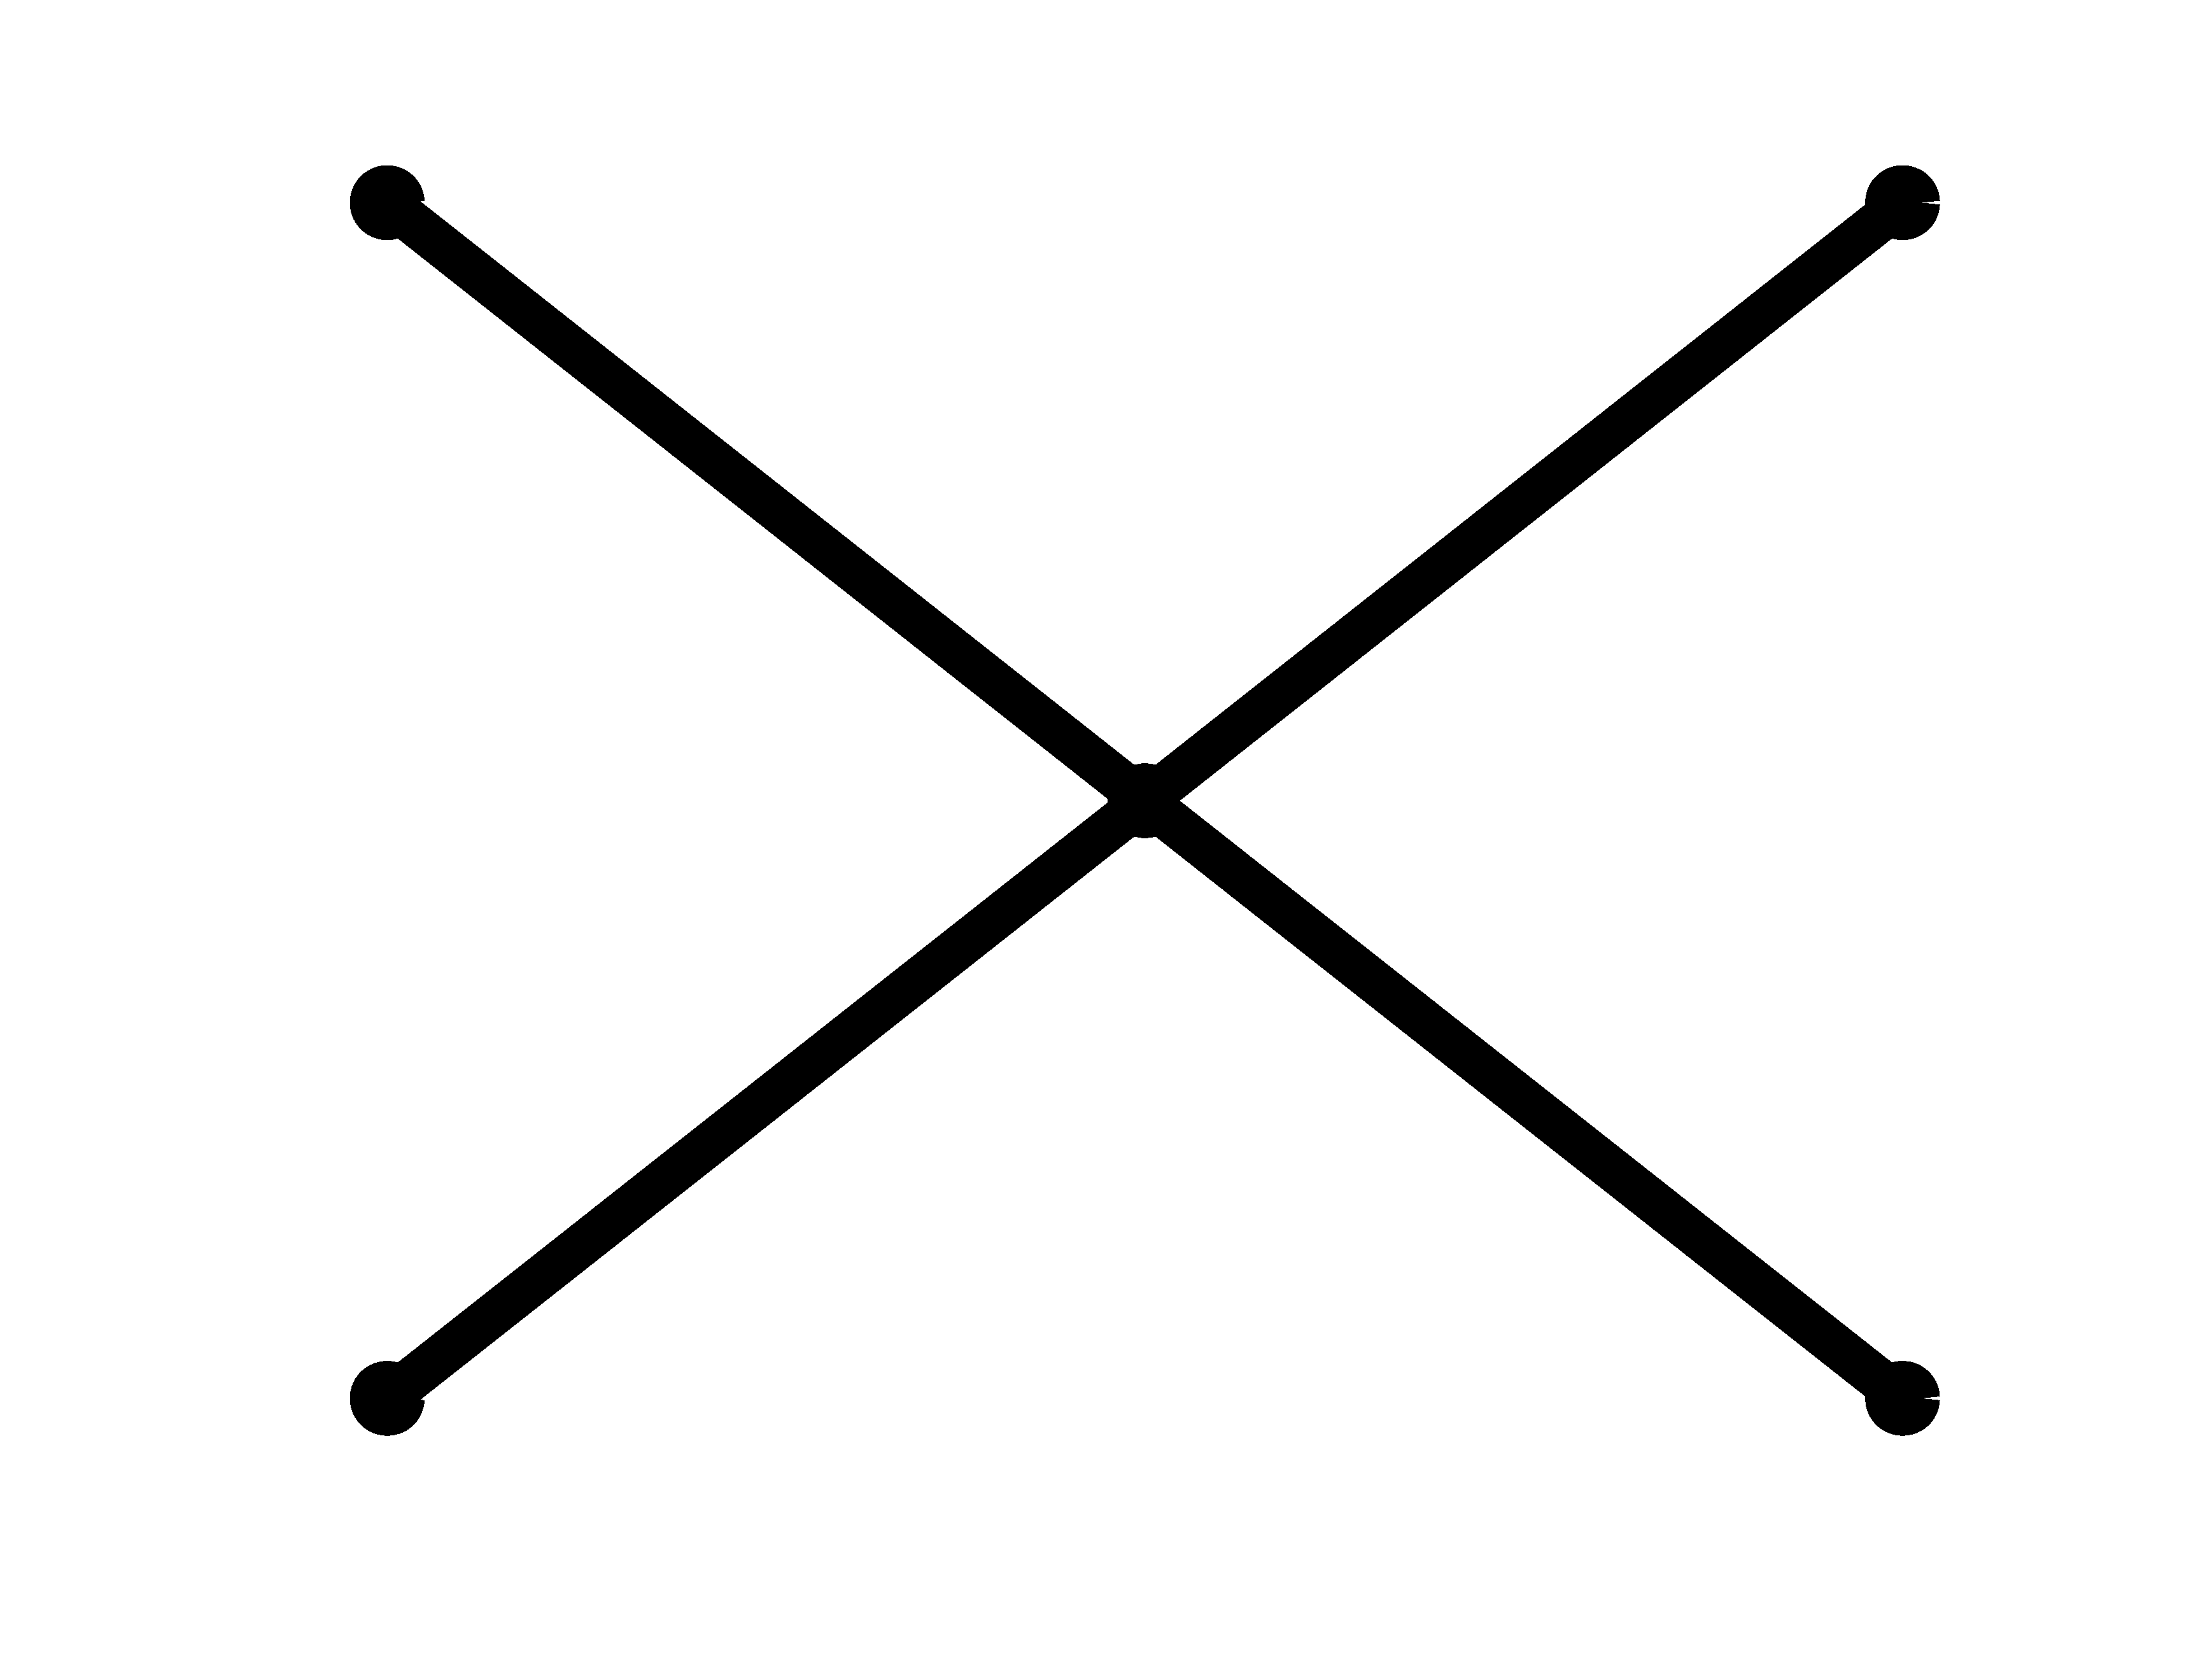
\epsfig{file = \fignet/Motif-Star4.eps, clip=, 
              width=0.05\textwidth}
          \end{tabular}   
        \end{tabular}  } \\
      \paragraph{Alternative strategy} proposed in \refer{MSB06}
    \end{tabular}
    &
    \begin{tabular}{c}
      %\hspace{-1cm}
      \epsfig{file= \figmotif/MotifStar4-Recouv3.eps,
        clip=, width=0.5\textwidth, height=0.8\textheight}
    \end{tabular}
  \end{tabular}  
  }

%==================================================================== 
\frame{ \frametitle{Choosing the model: FDD vs EDD}
  \paragraph{Case of the FDD model:} The number of star motifs
  $\mbf_k$ (with $k$ arrows) is given by the degrees of the nodes
  $d_i$:
  $$
  N(\mbf_k) = \sum_i \binom{d_i}{k}
  \qquad \Rightarrow \qquad
  \left\{
    \begin{array}{rcl}
      \Esp_{FDD}[N(\mbf_k)] & = & N_{\obs}(\mbf_k), \\
      \\
      \Var_{FDD}[N(\mbf_k)] & = & 0.
    \end{array}
  \right.
  $$\Pause

  \bigskip
  \paragraph{Expected degree distribution (EDD) model.} $\dbf_{\obs} =
  \{d_i\}_i$ degrees in the observed graph;
    \begin{eqnarray*}
    \{K_i\}_i \text{ i.i.d. } & \sim & \Ucal\{\dbf_{\obs}\} \\
    \{X_{ij}\} \text{ independent } | \{Z_i\}: X_{ij}  & \sim &
    \Bcal(c K_i K_j)
  \end{eqnarray*}
  \emphase{$\rightarrow$} Preserves the distribution of the degrees, \\
  \emphase{$\rightarrow$} Satisfies the stationarity assumption (H1).
  }

%====================================================================
\subsection{(Approximate) Distribution of the count}
%====================================================================
\frame{\frametitle{Compound Poisson approximation}
  \paragraph{Compound Poisson heuristic:} Motif occurrences appear in
  clumps
  \begin{eqnarray*}
    \text{Number of clumps } C & \sim & \Pcal(\lambda) \\
    \text{Clump sizes } \{S_c\}_c \text{ i.i.d.} & \sim & \Gcal(1-a) \\
    N(\mbf) & \overset{\Dcal}{\approx} & \sum_{c=1}^C S_c
  \end{eqnarray*}
  (inspired from sequence motifs: {\textcolor{blue}{\sl R. \&
  al. (2005)}}\nocite{RRS05}).

  \bigskip\bigskip
  \paragraph{Moment fit:} 
  $$
  a = \frac{\Var\Nm - \Esp\Nm}{\Var\Nm + \Esp\Nm}, \qquad
  \lambda = (1-a) \Esp\Nm.
  $$
  }

% %==================================================================== 
% \frame{ \frametitle{Some simulations}
%   \vspace{-.5cm}\hspace{-.5cm}
%   \begin{tabular}{p{.5\textwidth}p{.5\textwidth}}
%     \emphase{Motif $\Vsf$  (frequent)} 
%     & 
%     \emphase{Motif $\square$ (rare)} \\
%     \hspace{-.5cm}
%     \epsfig{file = \fignet/hist_200_0.005_0.5_0.1_V.eps,
%       width=.5\textwidth, height=.4\textheight, clip=} 
%     & 
%     \hspace{-.5cm}
%     \epsfig{file = \fignet/hist_200_0.01_0.1_0.1_C.eps,
%       width=.5\textwidth, height=.4\textheight, clip=} \\
%     \hspace{-.5cm}
%     \epsfig{file = \fignet/PPPlot_200_0.005_0.5_0.1_V.eps,
%       width=.5\textwidth, height=.4\textheight, clip=}      
%     &
%     \hspace{-.5cm}
%     \epsfig{file = \fignet/PPPlot_200_0.01_0.1_0.1_C.eps,
%       width=.5\textwidth, height=.4\textheight, clip=}  
%   \end{tabular}
%   }

%==================================================================== 
\frame{ \frametitle{Some simulations}
  \hspace{-.5cm}
  \begin{tabular}{cc}
    \begin{tabular}{p{.2\textwidth}}
      \paragraph{Mixture model}\\
      $K = 2$ \\
      $n = 200$ \\
      %$\overline{\gamma} = .5$ \\
      \\             
      \paragraph{Distributions}\\
      '$G$': Gaussian, \\
      '$CP$': compound Poisson \\
      \\ 
      \paragraph{Accuracy}  \\
      $D$: total variation distance, \\
      $\hat{F}$: actual level of the 99\% quantile.
    \end{tabular}\Pause
    &
    \begin{tabular}{p{.6\textwidth}}
      \emphase{Motif $\Vsf$  (frequent)} \qquad\qquad\qquad ($D$, $F$ in \%)
      {\small
        \begin{tabular}{c|c|c|c|c|c|c|c}
          $\Esp$ & $\mathbb{V}$ & $\lambda$ & $\frac{1}{1-a}$  & $D_G$ &
          $D_{CP}$ & 
          $\hat{F}_G$ & \emphase{$\hat{F}_{CP}$} \\ \hline
          159.5 & 2034.0 & 23.1 & 6.66 & 20.4 & 19.7 & 2.5 & \emphase{1.6} \\
          104.9 & 590.5  & 31.6 & 3.33 & 15.2 & 14 & 1.9 & \emphase{1.2}\\
          98.5  & 484.0  & 33.3 & 2.27 & 13.1 & 12.6 & 1.1 & \emphase{0.7}\\
          98.5  & 484.0  & 33.2 & 2.27 & 14.3 & 13.2 & 1.6 & \emphase{1.1}\\
          98.5  & 488.4  & 33.1 & 2.27 & 14.5 & 14.8 & 2.5 & \emphase{0.9}\\
        \end{tabular}
        }\Pause
      \\  \\
      \emphase{Motif $\square$ (rare)} \\
      {\small
        \begin{tabular}{c|c|c|c|c|c|c|c}
          $\Esp$ & $\mathbb{V}$ & $\lambda$ & $\frac{1}{1-a}$  & $D_G$ & $D_{CP}$ &
          $\hat{F}_G$ & \emphase{$\hat{F}_{CP}$} \\ \hline
          7.31&21.72&3.68& 2 &11.8&5.4&3.2&\emphase{0.9}\\
          2.57&3.42&2.21 & 1.16 &9.3&2.7&3.6&\emphase{0.5}\\
          2.74&3.69&2.33 & 1.17 &12.3&3.6&4.7&\emphase{1.2}\\
          1.94&2.40&1.74 & 1.11  &11.3&2.0&3.2&\emphase{1.6}\\
          2.74&3.72&2.32 & 1.17 &10.8&4.5&3.7&\emphase{0.7}\\
        \end{tabular}
        }
    \end{tabular}
  \end{tabular}
  }

%==================================================================== 
\frame{ \frametitle{{\sl E coli} regulatory network} 
  \paragraph{Comparison with 'Mfinder'}

  \begin{tabular}{ll}
    \hspace{-.5cm}
    \begin{tabular}{p{.5\textwidth}}
      \paragraph{Here} \\
      Occurrences: induced \\
      Model: mixture \\
      Distribution: compound Poisson
    \end{tabular}
    &
    \hspace{-.5cm}
    \begin{tabular}{p{.4\textwidth}}
      \paragraph{Mfinder} \\
      Occurrences: exact \\
      Model: FDD \\
      Distribution: Gaussian
    \end{tabular} 
    \\
    \\
    \hspace{-.6cm}
    {\small
    \begin{tabular}{crrrr}
      Motif & $N_{\obs}(\mbf)$ & $\Esp(N)$ & $\sigma(N)$ & $p$  \\              \hline
      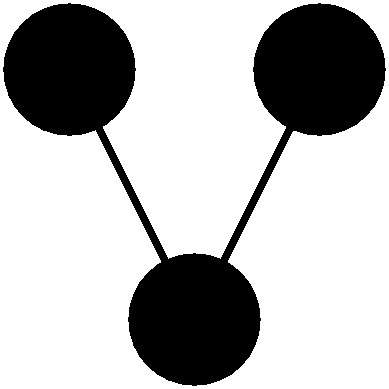
\epsfig{file = \fignet/Vmotif.eps, width=.3cm, clip=} &
      14\,113 & 13\,118 & 2\,599 & 3E${-1}$ \\ 
      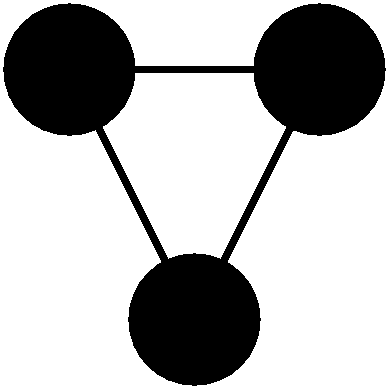
\epsfig{file = \fignet/trianglemotif.eps, width=.3cm, clip=}
      & 75 & 64.4 & 20 & 3E${-1}$ \\ 
      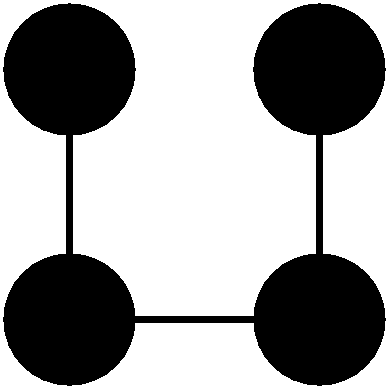
\epsfig{file = \fignet/chainmotif.eps, width=.3cm, clip=} &
      98\,697 & 90\,059 & 26\,064 & 3E${-1}$ \\ 
      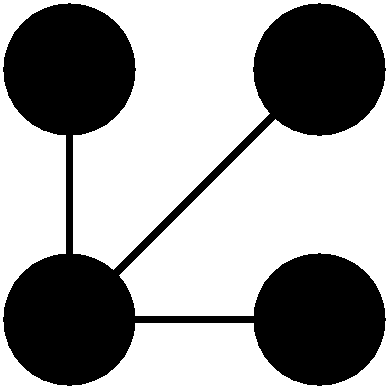
\epsfig{file = \fignet/starmotif.eps, width=.3cm, clip=} &
      112\,490 & 89\,372 & 26\,423 & 2E${-1}$ \\
      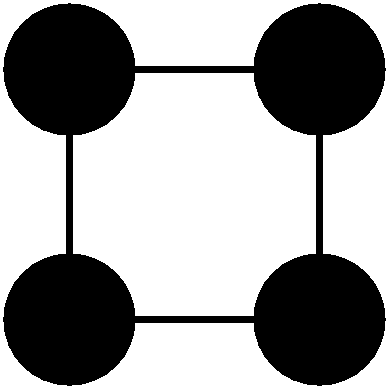
\epsfig{file = \fignet/squaremotif.eps, width=.3cm, clip=} &
      1\,058 & 492 & 202 & \emphase{1E${-2}$} \\ 
      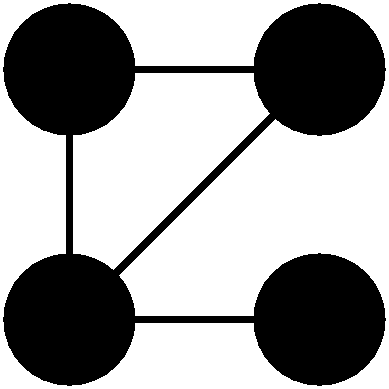
\epsfig{file = \fignet/whisker.eps, width=.3cm, clip=} &
      3\,535 & 2\,756 & 1\,087 & 2E${-1}$ \\ 
      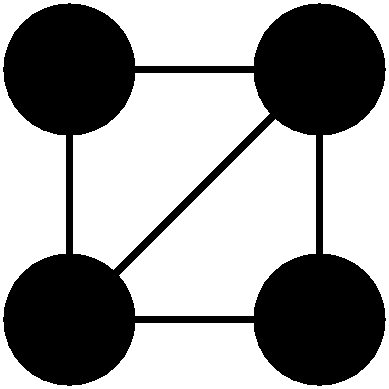
\epsfig{file = \fignet/halfclique.eps, width=.3cm, clip=} & 79 &
      33.2 & 19.5 & \emphase{3E${-2}$} \\ 
      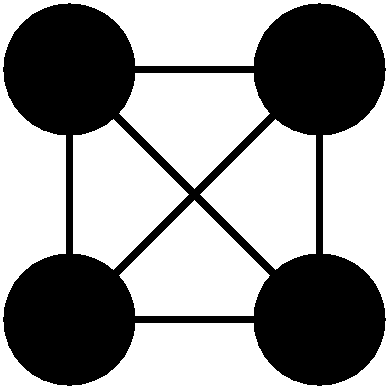
\epsfig{file = \fignet/clique.eps, width=.3cm, clip=} & 0 &
      0.165 & 0.432 & 1.00 \\ 
    \end{tabular}
    }
    &
    \hspace{-.6cm}
    {\small
    \begin{tabular}{rrrr} 
      $N_{\obs}(\mbf)$ &
      $\overline{N}_{100}$&$\overline{\sigma }_{100}$&
      $p$ \\
      \hline
      13\,888 & {13\,648} & \emphase{51.8} &  {2E${-6}$}    \\
      75      & {155}   & \emphase{17.3} & {2E${-6}$}     \\
      87\,869 & {112\,532} & {1\,957} & {1E${-36}$}  \\
      109\,113& {103\,186} & {1\,084} & {2E${-8}$}     \\
      979     & {796} & {64.7} & {2E${-3}$}    \\
      3\,219  & {8\,734} & {945} & {3E${-9}$}   \\
      79      & {273} & {66.7}& {2E${-3}$}    \\
      0       & {6.2} & {3.7} & {4E${-2}$}       
    \end{tabular}
    }
  \end{tabular}
  }

%====================================================================
\subsection{Perspectives}
%====================================================================
\frame{\frametitle{Network comparison: in progress} \Pause
  \paragraph{Aim:} Define a (dis-)similarity measure to compare
  networks. 

  \bigskip
  \paragraph{Strategy:} Define it based on network motif frequencies.

  \bigskip\bigskip\Pause
  \paragraph{Desirable properties:} avoid dependency on
  'irrelevant' characteristics, such as
  \begin{itemize}
  \item network sizes, 
  \item network densities, 
  \item colour frequencies in each network, 
  \item redundancy between motifs frequencies.
  \end{itemize}
  }

%====================================================================
\frame{\frametitle{Motif-based description}
  \paragraph{Vector of counts.} For a set of (coloured or topological)
  motifs $(\mbf_1, \dots, \mbf_M)$ and a given network $g$, define
  $$
  {\Nbf}_g = [{N}_g(\mbf_1) \; \dots \; {N}_g(\mbf_M)].
  $$

  \bigskip
  \paragraph{Moments.} For a series of random graph models
  --~satisfying (H1) and (H2)~--, we know how to compute
  \begin{itemize}
  \item means: 
    $$
    \Esp N_g(\mbf) \propto \binom{n_g}{k_\mbf} \mu_g(\mbf),
    $$
  \item variances: $\Var N_g(\mbf)$,
  \item covariances $\Cov[N_g(\mbf), N_g(\mbf')]$ (not shown).
  \end{itemize}

  \bigskip
  \paragraph{Idea:} Define a distance
  $$
  d(g, g') = f(\Nbf_g, \Nbf_{g'} | \Esp\Nbf, \Var\Nbf).
  $$
  }

% %====================================================================
% \frame{\frametitle{Normalised counts} 
%   To account for both \emphase{network and motif sizes}, we define 
%   $$
%   \tilde{N}_g(\mbf)  =  \binom{n_g}{k_\mbf}^{-1} N_g(\mbf)
%   \qquad \text{and} \qquad
%   \tilde{\Nbf}_g  =  [\tilde{N}(\mbf_1) \; \dots \;
%   \tilde{N}(\mbf_M)].
%   $$
% %   \begin{eqnarray*}
% %   \tilde{N}_g(\mbf) & = & \binom{n_g}{k_\mbf}^{-1} N_g(\mbf) \\
% %   \text{and} \qquad
% %   \tilde{\Nbf}_g & = & [\tilde{N}(\mbf_1) \; \dots \; \tilde{N}(\mbf_M)].
% %   \end{eqnarray*}

%   \bigskip
%   \paragraph{Moments of the normalised counts:}
%   $
%   \mubf_g := \Esp(\tilde{\Nbf}_g), 
%   \quad
%   \tilde{\Sigmabf}_g := \Var(\tilde{\Nbf}_g)
%   $
%   \begin{eqnarray*}
%     \Esp\tilde{N}_g(\mbf) & = & \binom{n_g}{k_\mbf}^{-1} \Esp N_g(\mbf)\\ 
%     \Var\tilde{N}_g(\mbf) & = & \binom{n_g}{k_\mbf}^{-2} \Var {N}_g(\mbf) \\
%     \Cov[\tilde{N}_g(\mbf), \tilde{N}_g(\mbf')] & = &
%     \binom{n_g}{k_\mbf}^{-1}\binom{n_g}{k_{\mbf'}}^{-1}
%     \Cov[{N}_g(\mbf), {N}_g(\mbf')] 
%   \end{eqnarray*}
%   }

% %====================================================================
% \subsection{A distance between networks}
% \frame{ \frametitle{Mahalanobis distance}
% %====================================================================
%   If networks $g$ and $g'$ are independent,
%   $$
%   \Esp(\tilde{\Nbf}_g - \tilde{\Nbf}_{g'}) = \mubf_g - \mubf_{g'}, 
%   \qquad
%   \Var(\tilde{\Nbf}_g - \tilde{\Nbf}_{g'}) = \tilde{\Sigmabf}_g +
%   \tilde{\Sigmabf}_{g'} 
%   $$

%   \bigskip
%   \paragraph{Cholevski decomposition:} Inverse covariance matrix as a
%   metric accounting for correlations:
%   $$
%   \Var\left[\left(\tilde{\Sigmabf}_g +
%       \tilde{\Sigmabf}_{g'}\right)^{-1/2}(\tilde{\Nbf}_g -
%     \tilde{\Nbf}_{g'})\right] = {\bf I}
%   $$
  
%   \bigskip
%   \paragraph{Mahalanobis distance:} (cf LDA)
%   $$
%   d^2(g, g') = \|\tilde{\Nbf}_g - \tilde{\Nbf}_{g'}
%   \|^2_{\left(\tilde{\Sigmabf}_g + \tilde{\Sigmabf}_{g'}\right)^{-1}}.
%   $$
%   }

% %====================================================================
% \frame{ \frametitle{Descriptive analyses}
%   \paragraph{All distance-based data analysis} techniques can then be
%   applied. 

%   \Pause\bigskip
%   \begin{tabular}{cc}
%     \hspace{-0.5cm}
%     \begin{tabular}{p{.5\textwidth}}
%       \paragraph{Multidimensional scaling} ($\approx$ PCA) \\
%        \epsfig{file =
%          \fignet/motusOrganismsMahalanobisDistanceMatrix-MDS.eps,
%          angle=270, clip=, width=.5\textwidth}  
%     \end{tabular} \Pause
%     &
%     \hspace{-0.5cm}
%     \begin{tabular}{p{.5\textwidth}}
%       \paragraph{Distance based clustering} \\
%        \epsfig{file =
%          \fignet/motusOrganismsMahalanobisDistanceMatrix-HClust.eps,
%          angle=270, clip=, width=.5\textwidth}   
%     \end{tabular}
%   \end{tabular}
%   and more
%   \begin{itemize}
%   \item contribution of each motif to the distance, 
%   \item ...
%   \end{itemize}
%   }

% %====================================================================
% \frame{ \frametitle{Hypothesis testing}
%   \begin{tabular}{cc}
%     \hspace{-.5cm}
%     \begin{tabular}{p{.5\textwidth}}
%       \paragraph{Null hypothesis:}
%       $$      
%       \Hbf_0 = \{\mubf_g = \mubf_{g'}\}
%       $$

%       \paragraph{Test statistic:} 
%       $$
%       T = \frac1M d^2(g, g')
%       $$
      
%       \paragraph{Question:} Distribution of $T$
%       under $\Hbf_0$? $\Fcal_{M, \nu}$? \\
%     \end{tabular}
%     &
%     \begin{tabular}{p{.45\textwidth}}
%     \hspace{-.5cm}
%       \epsfig{file =
%       \fignet/MahalanobisHist_EstimatedParam_p0.1_AllMotifsSize3.ps,
%       clip=, width=.45\textwidth} 
%     \end{tabular}
%   \end{tabular} \\
%   (Work in progress by \textcolor{blue}{\sl L. Benaroya}) 
%   }

% %==================================================================== 
% \frame{ \frametitle{Some open questions}
%   \paragraph{(Asymptotic) distributions}
%   \begin{itemize}
%   \item of the counts $N(\mbf)$,
%   \item of the distance $d(g, g')$,
%   \end{itemize}
%   for non-naive random graph models?

%   \bigskip\bigskip
%   \paragraph{(Asymptotic) distributions}
%   \begin{itemize}
%   \item of the counts $N(\mbf)$,
%   \item of the distance $d(g, g')$,
%   \end{itemize}
%   for non-naive random graph models?

%   \bigskip\bigskip
%   \paragraph{But most of all:} what is the relevent graph model?
%   }

  \begin{tabular}{cc}
    \hspace{-.5cm}
    \begin{tabular}{p{.5\textwidth}}
    \end{tabular}
    & 
    \hspace{-.5cm}
    \begin{tabular}{p{.5\textwidth}}
    \end{tabular}
  \end{tabular}

%%% Local Variables: 
%%% mode: latex
%%% TeX-master: "StatSud"
%%% End: 
